%%% lorem.tex --- 
%% 
%% Filename: lorem.tex
%% Description: 
%% Author: Ola Leifler
%% Maintainer: 
%% Created: Wed Nov 10 09:59:23 2010 (CET)
%% Version: $Id$
%% Version: 
%% Last-Updated: Tue Oct  4 11:58:17 2016 (+0200)
%%           By: Ola Leifler
%%     Update #: 7
%% URL: 
%% Keywords: 
%% Compatibility: 
%% 
%%%%%%%%%%%%%%%%%%%%%%%%%%%%%%%%%%%%%%%%%%%%%%%%%%%%%%%%%%%%%%%%%%%%%%
%% 
%%% Commentary: 
%% 
%% 
%% 
%%%%%%%%%%%%%%%%%%%%%%%%%%%%%%%%%%%%%%%%%%%%%%%%%%%%%%%%%%%%%%%%%%%%%%
%% 
%%% Change log:
%% 
%% 
%% RCS $Log$
%%%%%%%%%%%%%%%%%%%%%%%%%%%%%%%%%%%%%%%%%%%%%%%%%%%%%%%%%%%%%%%%%%%%%%
%% 
%%% Code:



\chapter{Theory}
The following chapter describes the necessary information needed to solve the problem description and to help design an appropriate method. The theoretical part will first explain the concept of an agar plate, followed by various existing approaches to image processing and edge identification. 
\\

\section{Agar Plate}
Agar plates are Petri dishes containing agar, which is a gelatinous substance derived from red algae used as a bacteria growth medium. Agar plates are often used in laboratory settings to analyze if certain bacteria exist within a sample. Depending on the situation, the agar plate could be divided into multiple compartments, as shown in \textit{Figure \ref{fig:agar plate}}. Each compartment can be used to test different samples or the same sample with different bacteria.


% to reference a figure \ref{label}

%\begin{figure}[H]
%  \includegraphics[scale=1.7]{birds.jpg}
%  \caption{The birds}
%  \label{fig:birds}
%\end{figure}
    \begin{figure}[H]
        \begin{center}
            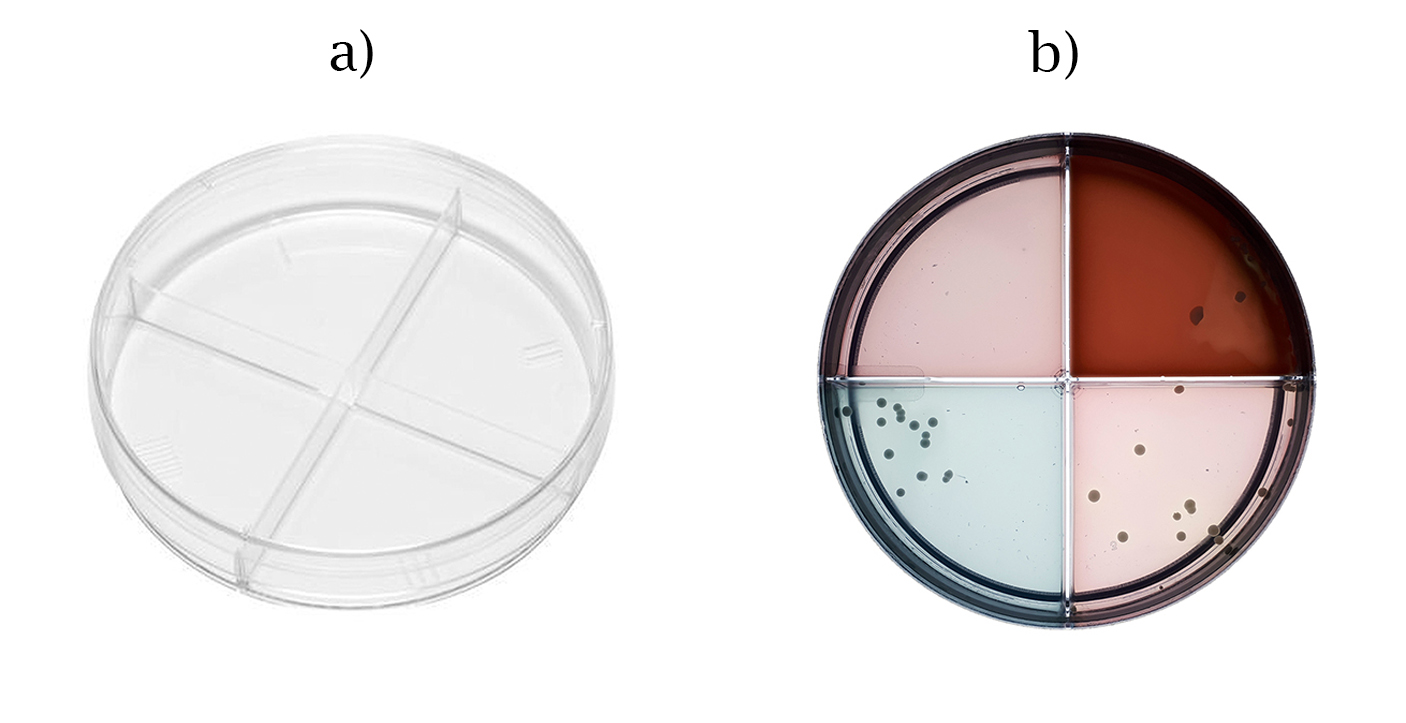
\includegraphics[width=.7\linewidth]{figures/petri.jpg}\\
            \caption{ a) Empty Petri dish with four compartments. b) Petri dish with agar, i.e., an agar plate.}
            \label{fig:agar plate}
        \end{center}
    \end{figure}

\section{Image Processing}

\noindent Digital image processing is about manipulating pixels. For example, improving, analyzing, or in some way, extracting information from an image. This section will focus on this type of algorithms and techniques, focusing on techniques suitable for the aim of the work.

%\section{Brightness and contrast}
\subsection{Color correction}
Altering the color of an image is an essential task in image processing and often means removing a dominant and undesirable color in a picture. Objects may have different colors on the images compared to reality. \\

\noindent \cite{Limare} proposes a color balance algorithm named Simplest Color Balance (SCB). The algorithm works by stretching red, green, and blue values within a [0, 255] range. High values are assumed to be white, and low values black. An image with low brightness, for example, may not have any pixels close to 255. By stretching the color scale [0, 255], the brightness can be increased or decreased. 


\subsection{Edge detecting}
\noindent Edges (i.e., an abrupt change of gray or color intensity) need to be distinguished in order to extract specific data of objects in images. By minimizing the number of false edges, often caused by image noise,  actual edges could easier be identified. If the goal is to find the most intense edge, as the edge of an agar plate, blur filters and morphological operations could be used as an extension. The Hough Transform algorithm (see \textit{Section 2.2.2.6}) is designed to find simple shapes within an image and to extract the coordinates or the area of an object.



\subsubsection{Canny Edge Detection}
The Canny operator\cite{Xuan} is based on a multi-stage algorithm initially developed to detect edges in images. Canny is divided into five different stages explained below. \\

\noindent \textbf{Gaussian Blur}\\
The first stage of Canny is to apply a Gaussian blur filter to reduce any image noise occurring, as shown in \textit{Figure \ref{fig:gaussian blur}}. Otherwise, pixel noise could be falsely detected as an edge. The algorithm uses a kernel, which is a convolution matrix of $n*n$ pixels, to search all pixels in an image. Each pixel is evaluated, and its pixel value is replaced with a weighted mean of its neighboring pixels. A two-dimensional Gaussian function is generally used to remove image noise (see \textit{Equation 2.1}). \begin{equation} G(x,y)=exp[-(x^2+y^2/2\sigma^2]/2\pi\sigma^2\end{equation} Where $\sigma$ (sigma) is the parameter that controls the smoothing extent of an image. 

\begin{figure}[H]
        \centering
        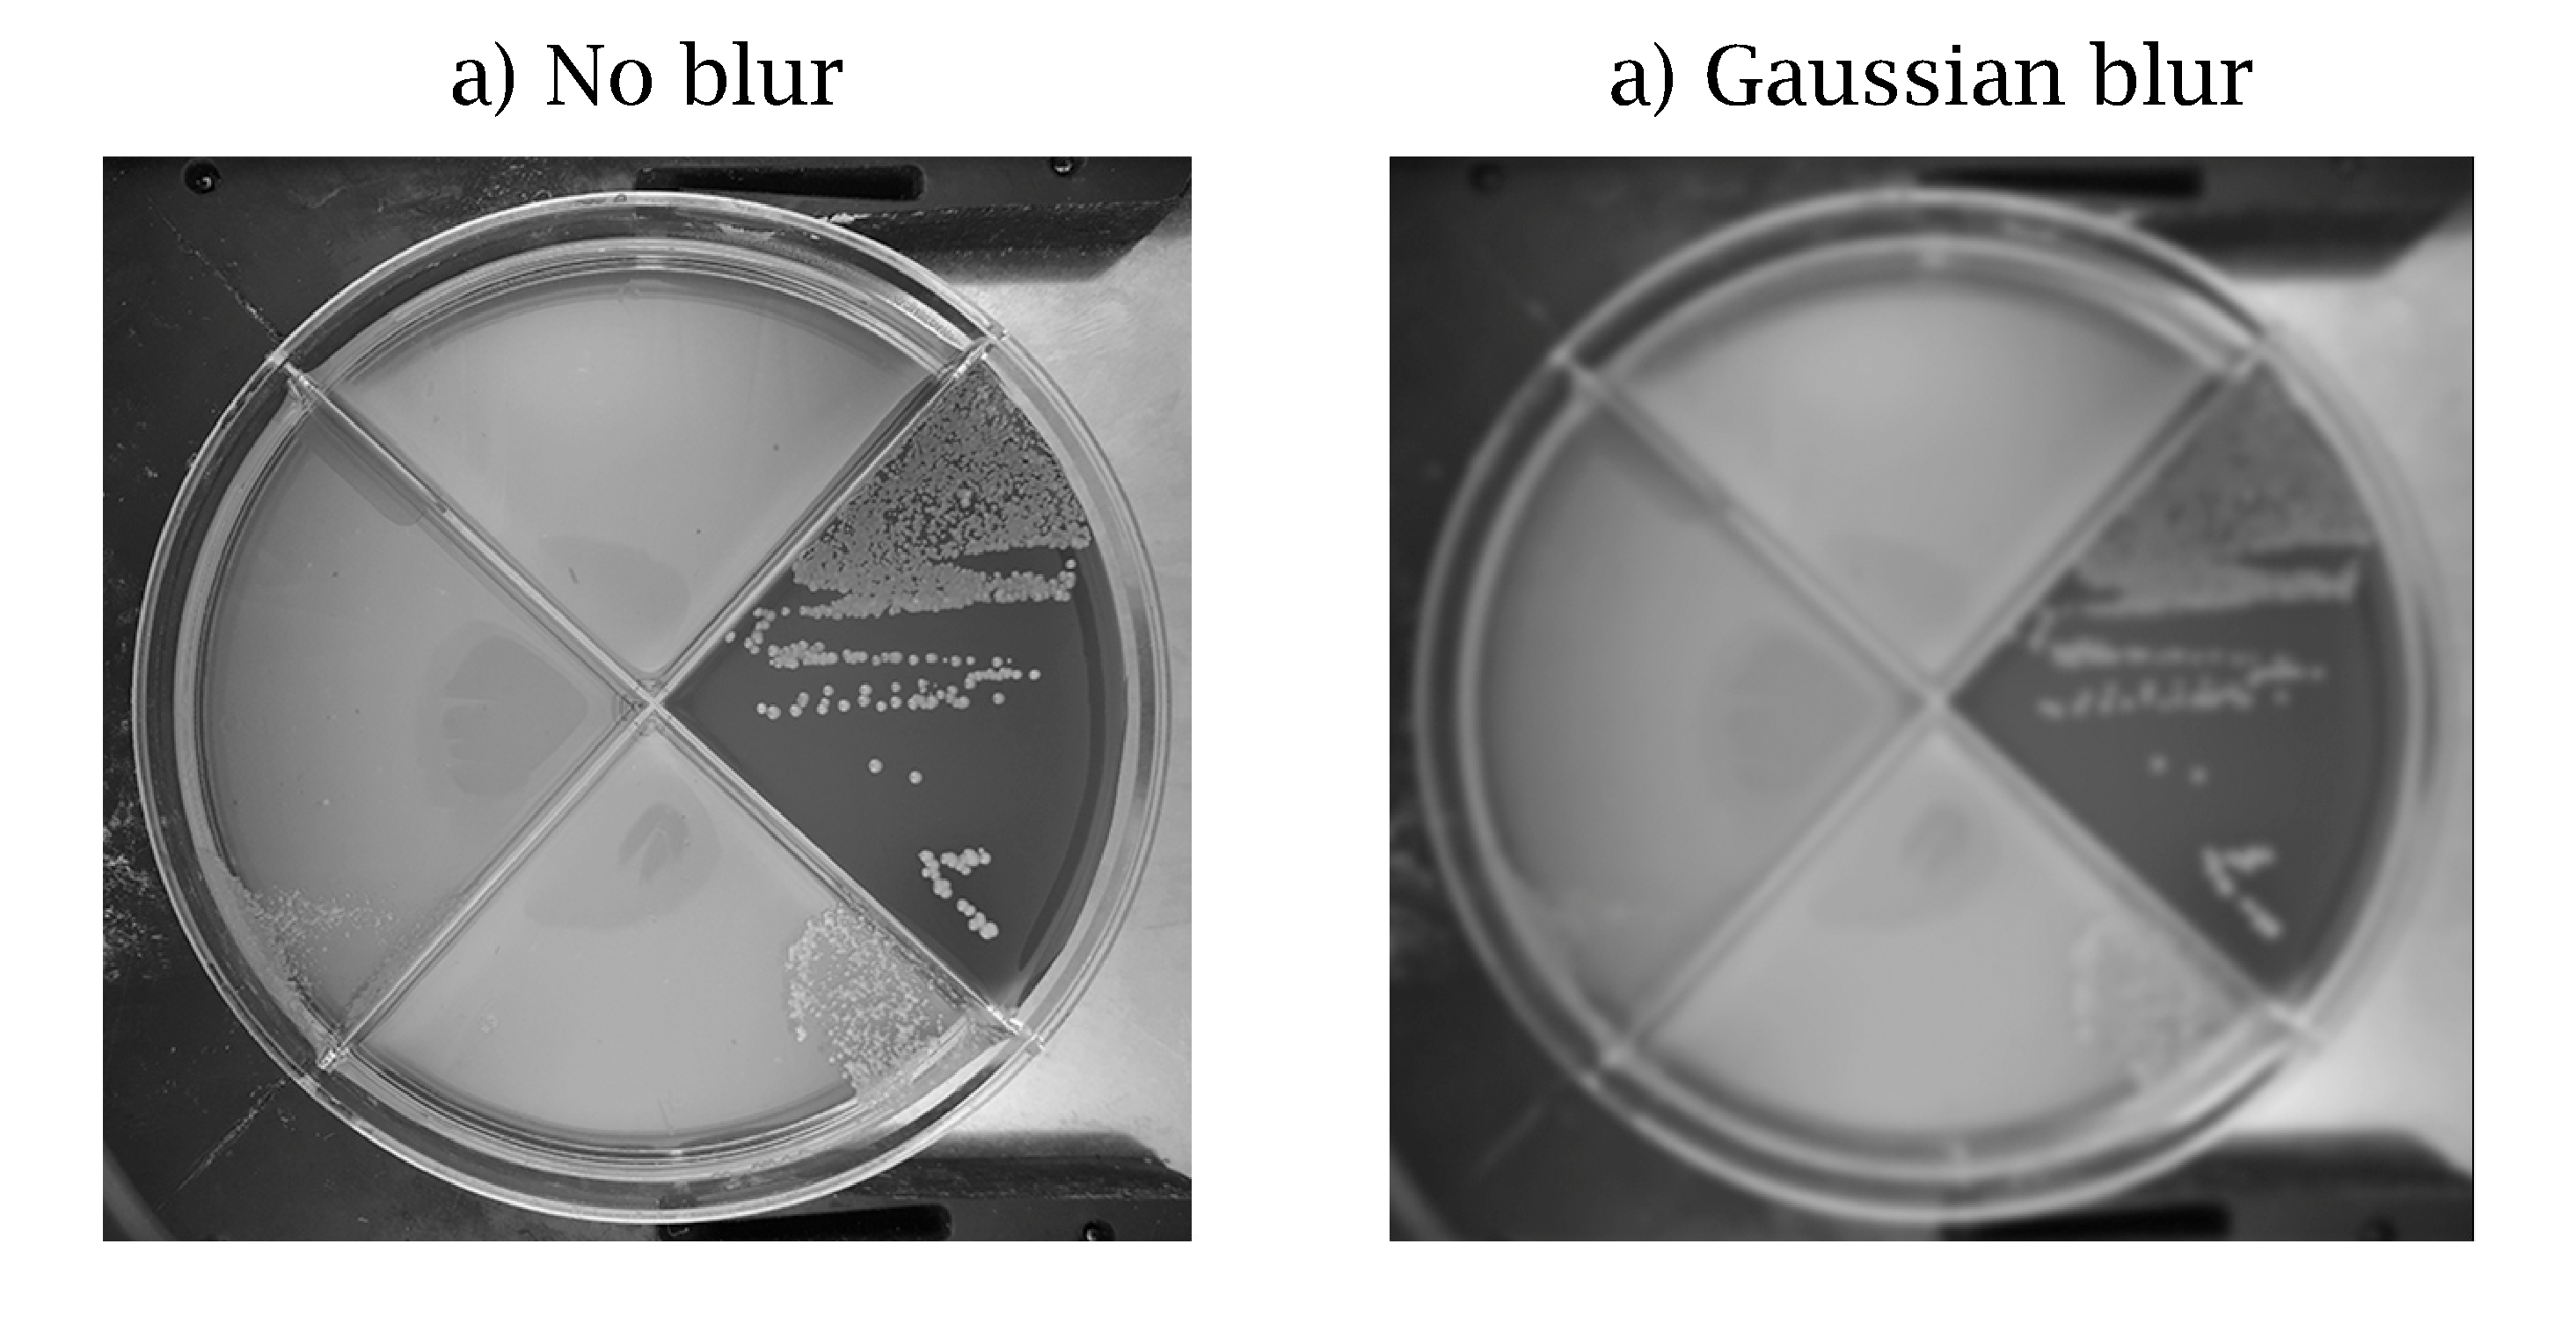
\includegraphics[width=.7\linewidth]{figures/PDF/Gaussian_blur.pdf}\\
        \caption{a) Before applying Gaussian Blur. b) After applying Gaussian Blur}
        \label{fig:gaussian blur}
\end{figure}\\

\noindent \textbf{Sobel Operator}\\
\noindent After the applied blur, a Sobel kernel is used to identify all intensity gradients. With its kernel, Sobel looks for areas in the image that have a high gradient, i.e., a distinct and sudden change in color (in RGB) or brightness (in grayscale). \textit{Figure \ref{fig:sobel kernel}} shows how the method works in the x-axis as well as the y-axis. Each value within the kernel is multiplied by the value at the corresponding location in the image. The sum of the matrix gives a gradient value. A higher value means a more defined edge. The derivative of the respective edges is then calculated to determine the angle of the edge.\\

\begin{figure}[H]
        \centering
        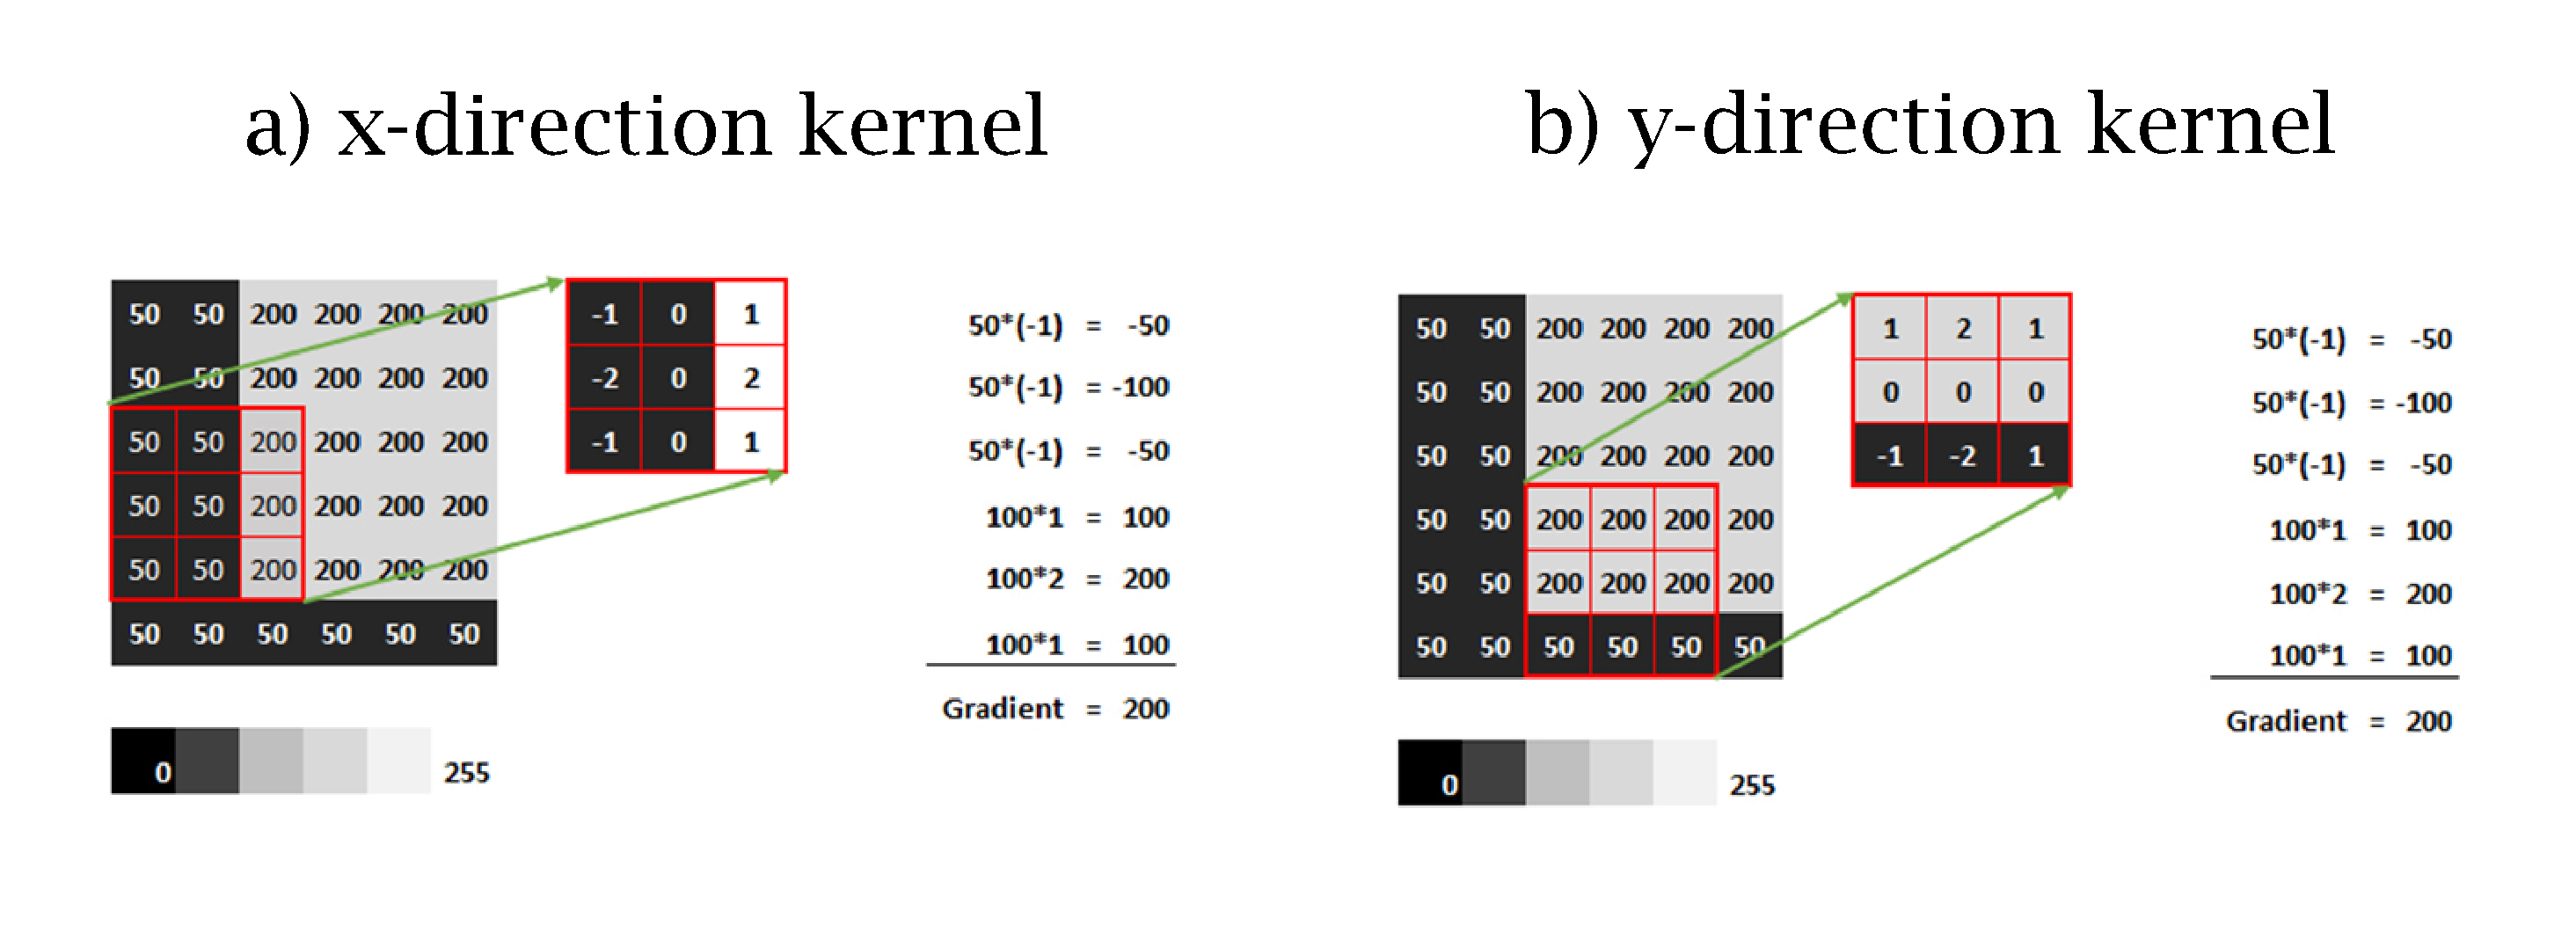
\includegraphics[width=1\linewidth]{figures/PDF/Sobel_kernel.pdf}
        \caption{The Sobel y-kernel checks for the gradient on the y-axis}
        \label{fig:sobel kernel}
\end{figure} \\\\

\noindent \textbf{Non-maximum suppression}\\
\noindent While the Sobel filter finds most edges, usually, only the most prominent are interesting. The output may have both thick and thin edges, and a non-maximum suppression can be used to sort out any false edges. \\

\noindent By using the gradient intensity matrix determined in the previous step, the algorithm seeks through the image, following the direction of the edge. For each pixel, the algorithm checks neighboring pixels to the left and right of the edge. If a neighboring pixel in the same direction is more intense than the current pixel, the most intense pixel is kept. \textit{Figure \ref{fig:canny suppression}} shows an example where the pixels with intensity values 170 and 115 would be dismissed, and 255 kept.\\

\begin{figure}[H]
    \centering
     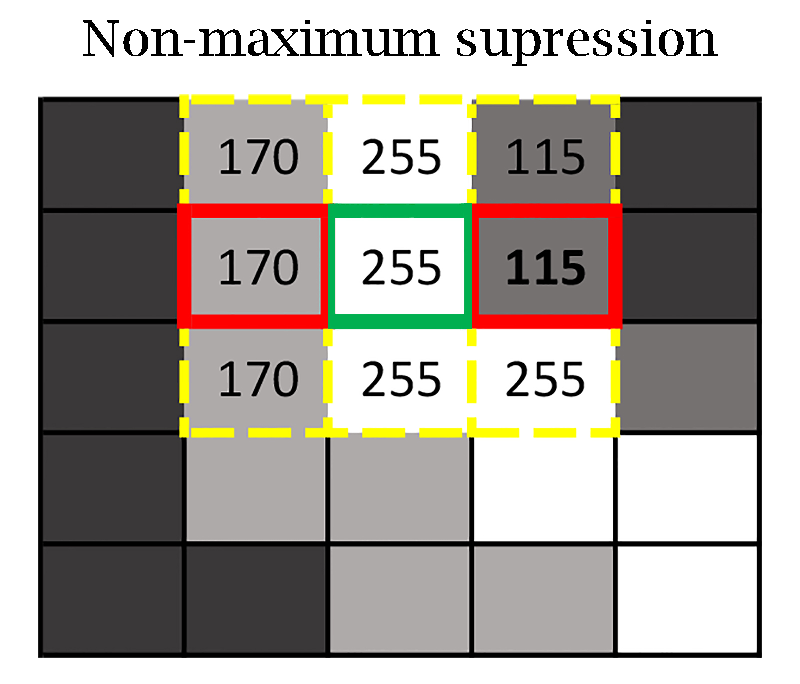
\includegraphics[width=.37\linewidth]{figures/PDF/Suppresion.pdf}\\
    \caption{Non-maximum suppression illustration. Values in red are dismissed, and green kept.}
    \label{fig:canny suppression}
\end{figure}

\noindent \textbf{Double threshold}\\
\noindent The non-maximum suppression will keep the most intense pixels identified in each edge, but there can still be intensity variations between these pixels. A lower and upper threshold is applied to strengthen the edge, which checks for pixels that are strong, weak, or non-relevant. The lower threshold is used to identify non-relevant pixels, while the upper threshold searches for strong pixels. Any pixels between the lower and upper threshold are marked as weak and will later be processed in the Hysteresis mechanism.\\ 

\noindent \textbf{Hysteresis}\\
\noindent The last stage of the Canny process is to decide which edges are true or not. With user-defined min and max parameters of a new threshold, previously detected weak pixels are transformed to strong pixels only if their pixel value is within the defined threshold range. \texit{Figure \ref{fig:hysteresis} b)} illustrates this procedure by discarding non-relevant pixels to value 0. The identified pixel also needs to be connected to a known edge, or else it will be discarded. \\

\begin{figure}[H]
    \centering
    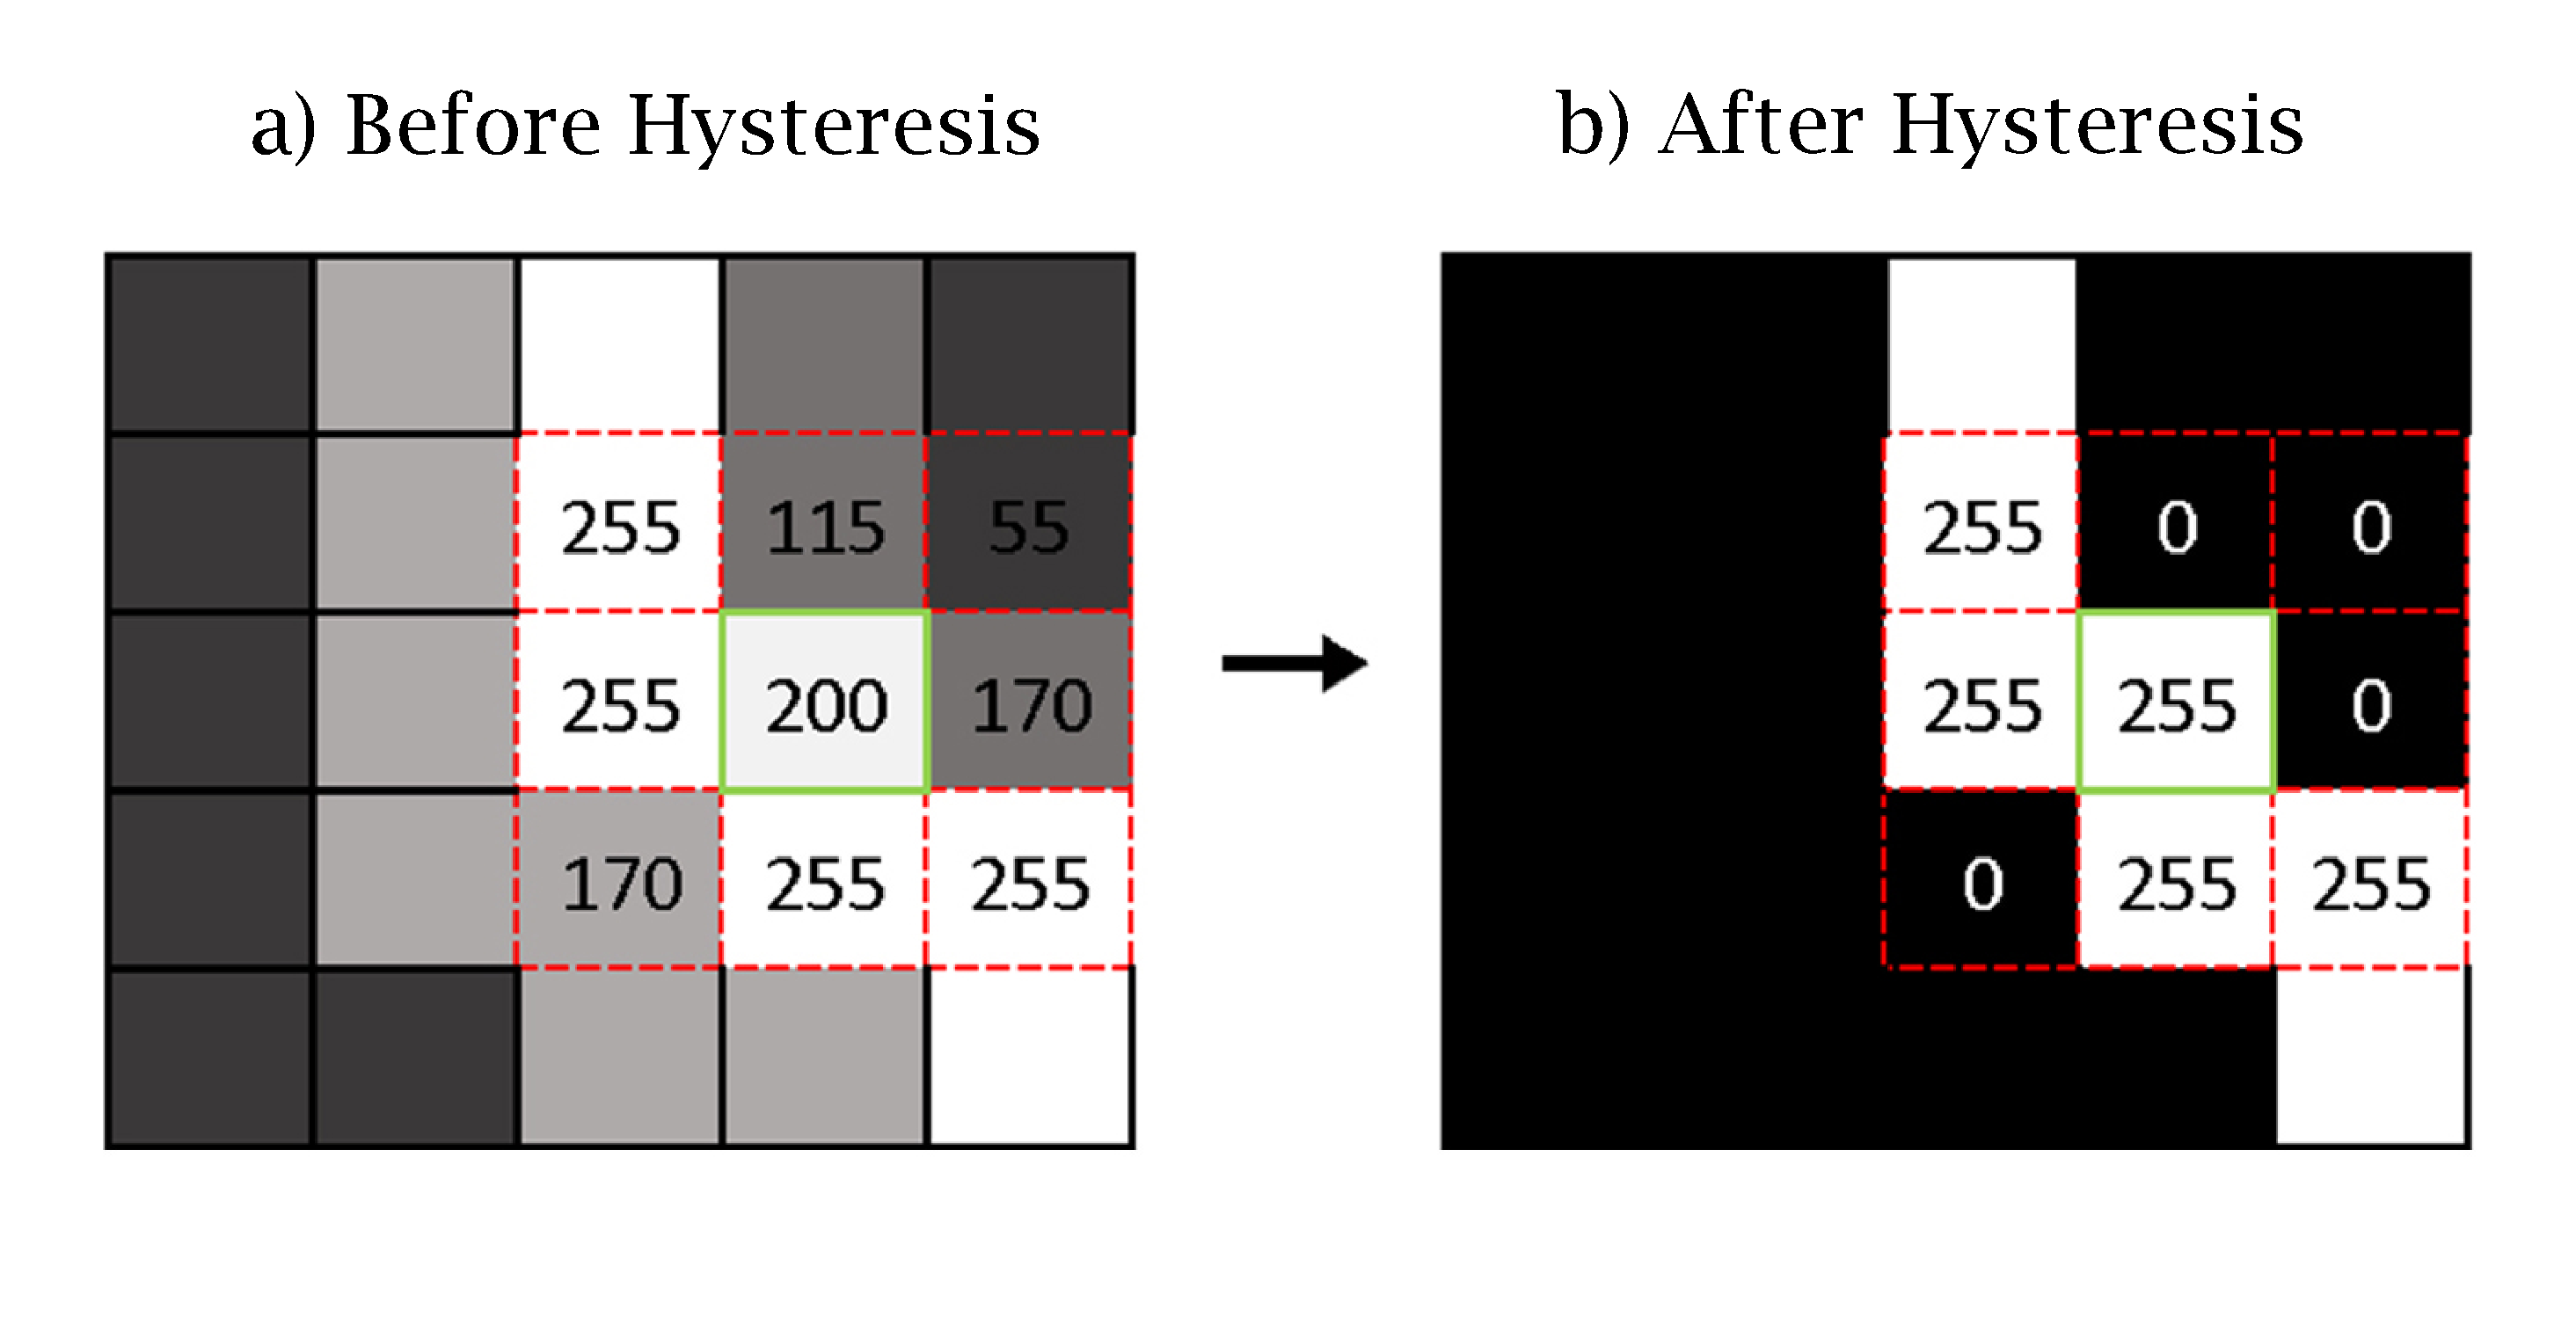
\includegraphics[width=.65\linewidth]{figures/PDF/Hysteresis.pdf}
    \caption{a) Before Hysteresis, b) after Hysteresis.}
    \label{fig:hysteresis}
\end{figure}

\subsubsection{Morphological Operations}
Morphological operations are used to process images based on geometrical structures. Different operations can be used to fix broken edges or areas within or outside the given boundaries of an object. The most common morphological operations are \textit{Dilation} and \textit{Erosion}\cite{Raid}, which either adds or removes pixels from an object contour. Dilation, followed by erosion, is called \textit{Closing}, which can be used to repair disconnected edges. Its counterpart \textit{Opening} are instead erosion followed by dilation can instead be used to reduce image noise \\

\noindent A structuring element (a matrix of user-defined size), searches the image checking each pixel with its corresponding neighbor (see \texit{Figure \ref{fig:dilate and erode}}). The value of each pixel within the structuring element is then decided based on different rules. For the dilation, each pixel is set to the most intense value found within the structuring element, while erosion sets each pixel values to the least intense. 

\begin{center}
\begin{figure}[H]
    \centering
    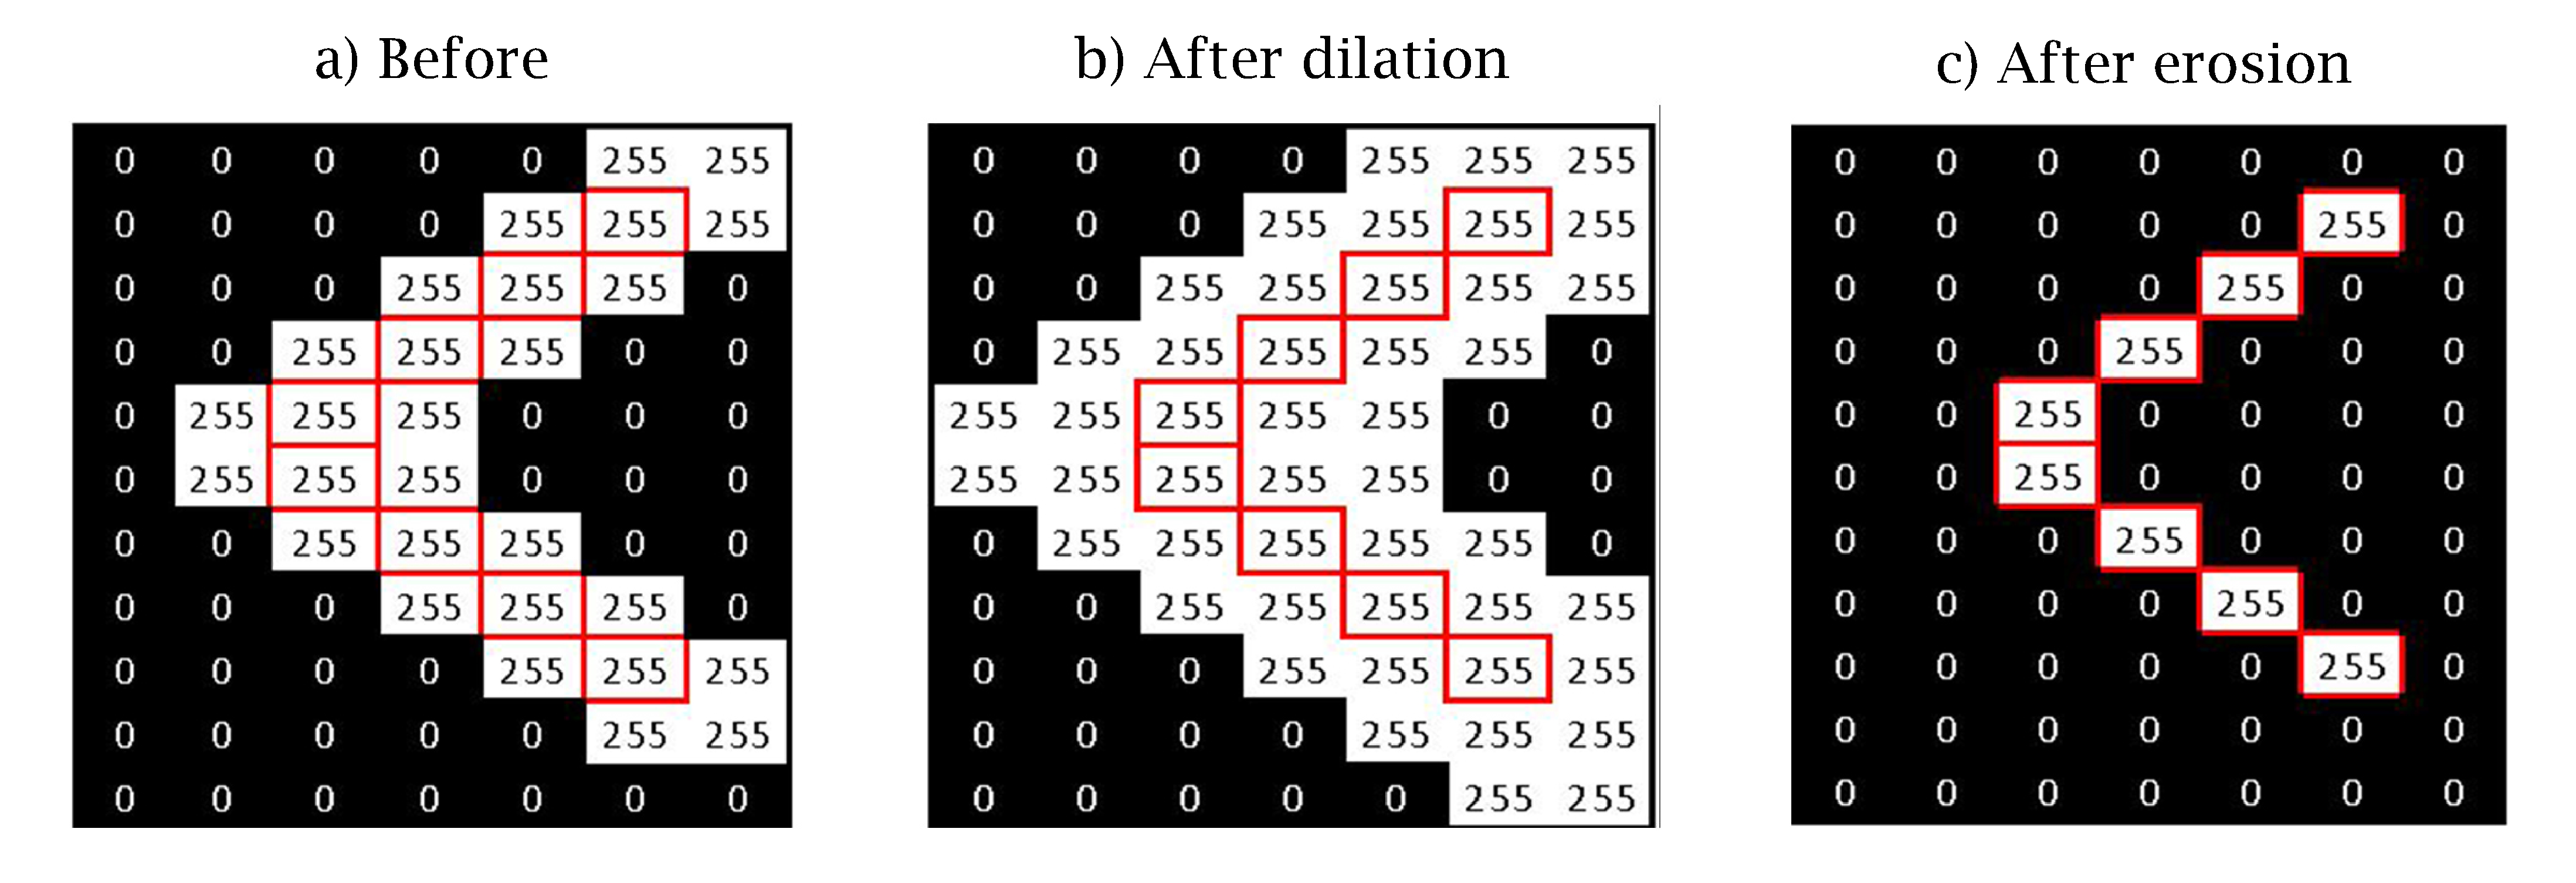
\includegraphics[width=1\linewidth]{figures/PDF/Morphological_dilate_erode.pdf}\\
    \caption{Dilation adds pixels to the object contour, while erosion
    removes pixels.}
    \label{fig:dilate and erode}
\end{figure}
\end{center}

\subsubsection{Skeletonize}
\textit{Skeletonization}\cite{Rakesh} is a technique that modifies a binary image using Dilation and Erosion to reduce foreground regions into a skeletal remnant, i.e., the innermost contour of a binary object (see \textit{Figure \ref{fig:skeletonize}}). In an ideal case, the result should give a 1-pixel-wide representation. By skeletonizing an image, one can achieve improved computation speed in image processing with only a light skeleton to process, as well as increased accuracy of finding the actual position of a line or edge.

\begin{figure}[H]
    \centering
    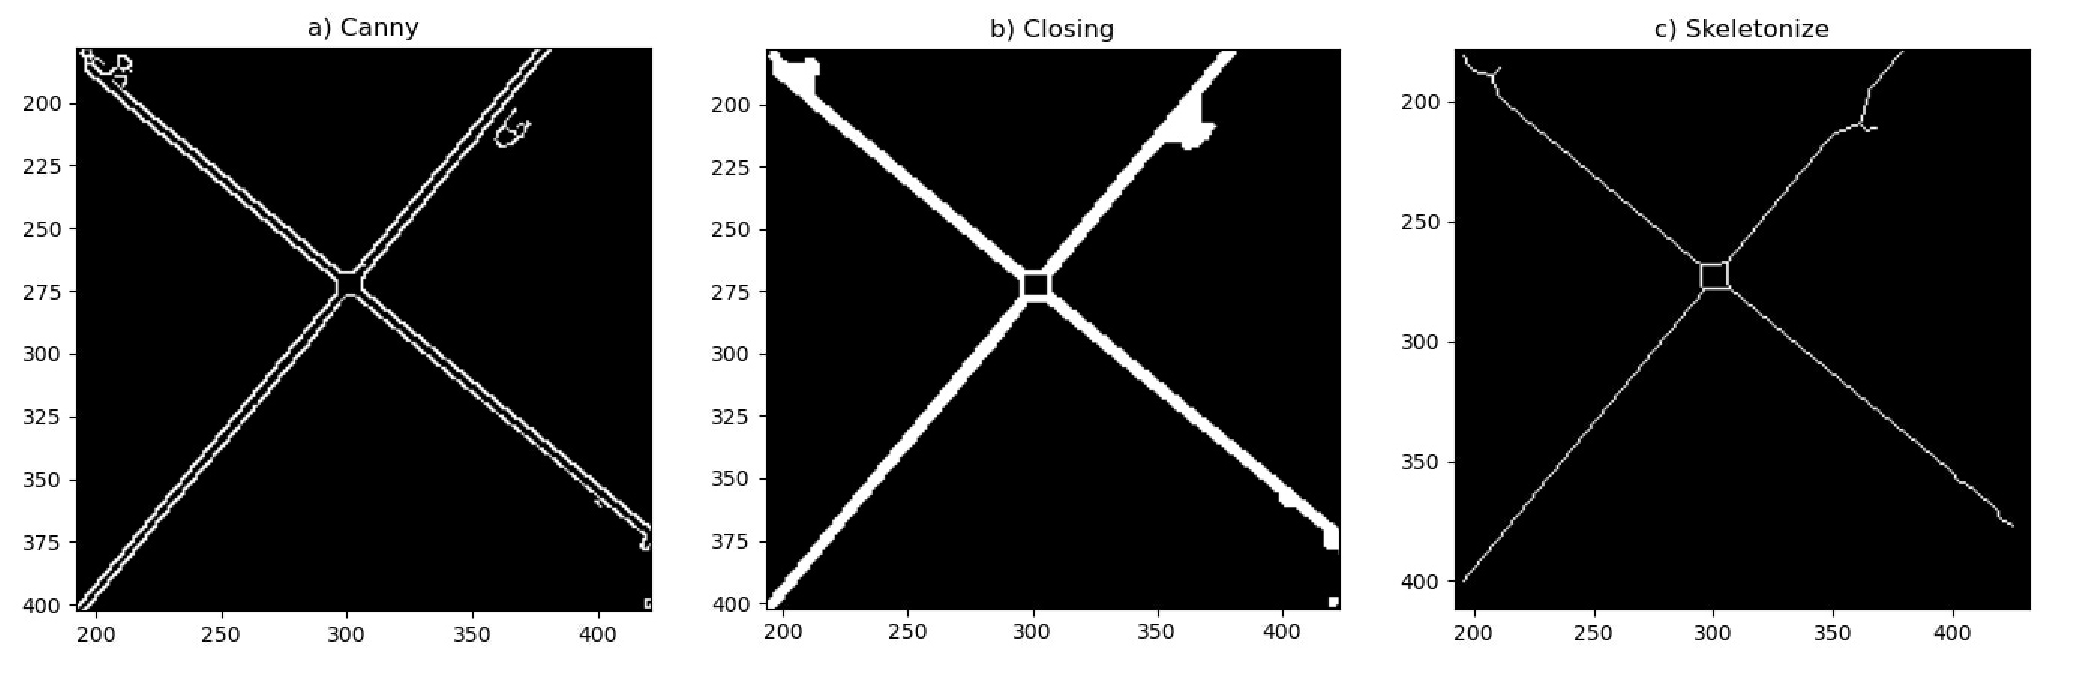
\includegraphics[width=0.8\linewidth]{figures/PDF/Skeletonize.pdf}\\
    \caption{The right image shows the output of a skeletonized binary image.}
    \label{fig:skeletonize}
\end{figure}

\noindent Opening is used to reveal the skeleton of an object. The process is repeated as long as the connectivity of the binary object is not broken. When broken, the last successful iteration is saved as output.

\subsubsection{Border following}
Extracting the contour of an object can be useful to analyze shapes and detect or recognize different objects. Border following \cite{Suzuki} is a type of algorithm that makes it possible to extract contours of given objects. Contours are generally defined by a closed curve joining the continuous points of an object boundary. For a contour to be identified, the object boundary should consist of pixels with the same color or intensity. 
For binary images, contours are divided into 1- and 0-components, which represent areas of their respectively binary image value. In \textit{Figure \ref{fig:suzuki border}}, $S_{1}$, which is the background 0-component, is interpreted as a hole between the frame border and the $B_{1}$ border. The algorithm checks images for 1-component and defines its borders as the transition between any 1-components neighboring 0-component.

\begin{figure}[H]
    \centering
     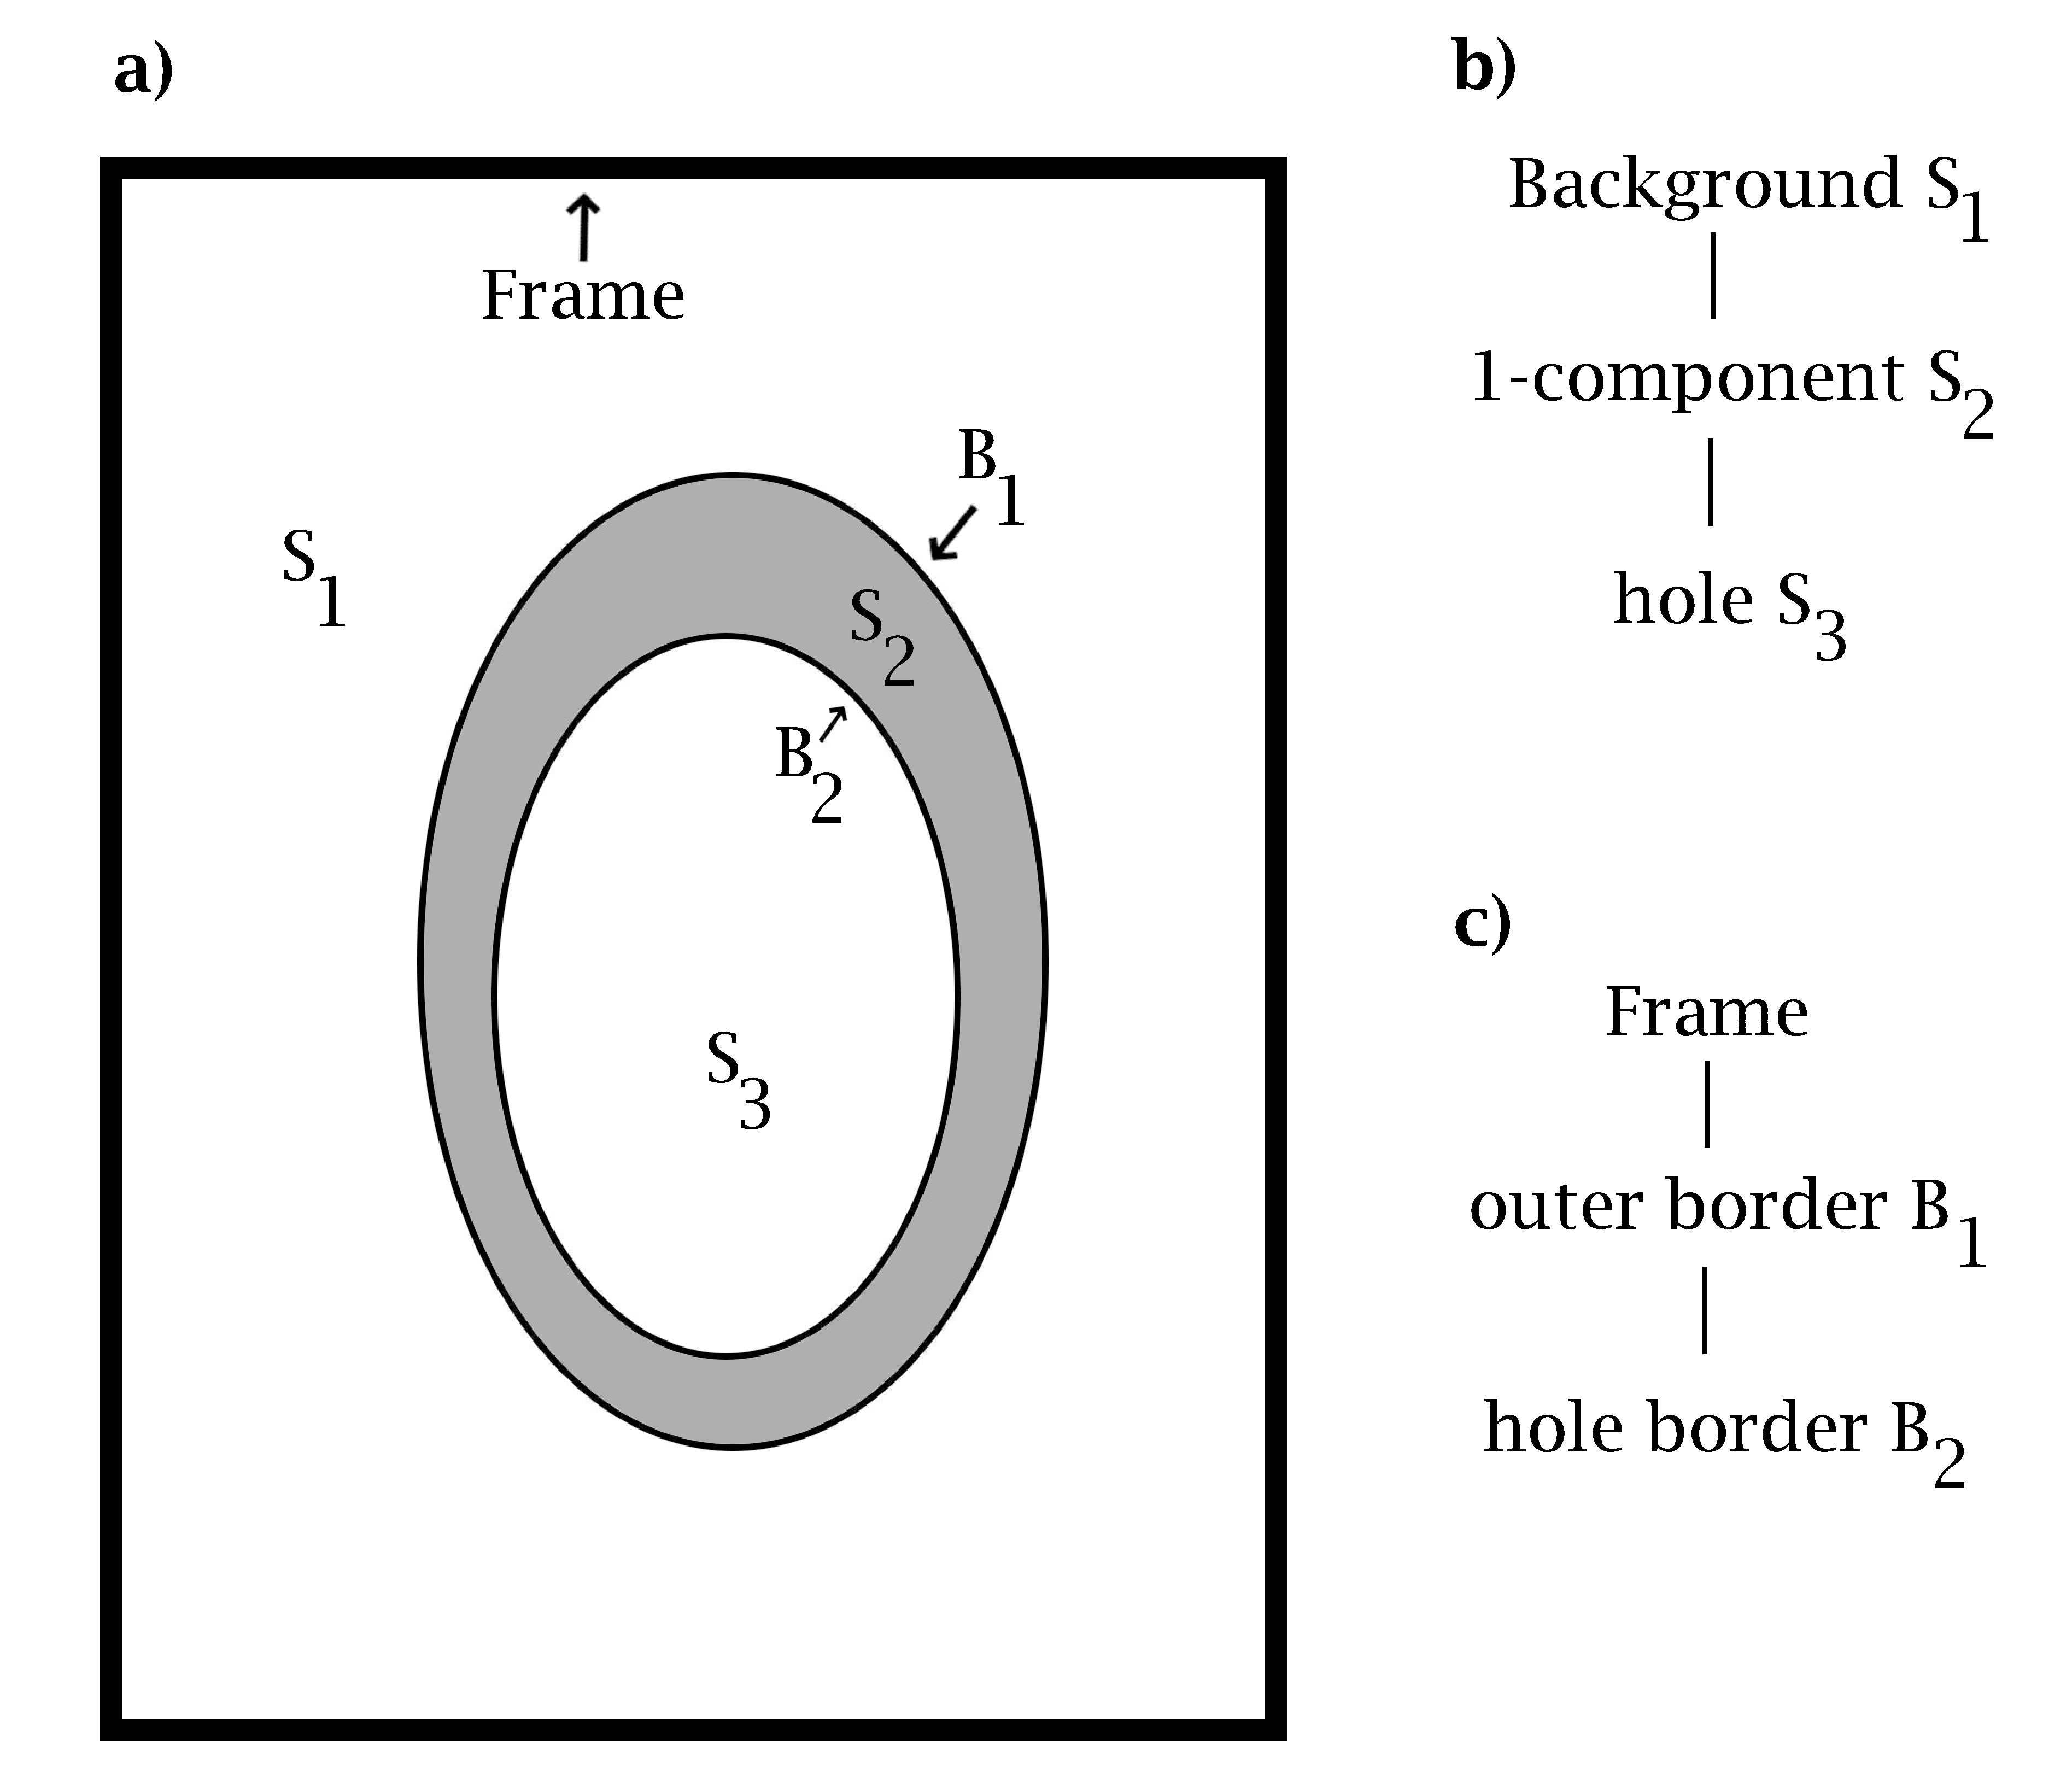
\includegraphics[width=0.65\linewidth]{figures/PDF/Border_following.pdf}
    \caption{a) Illustrates $S_{2}$ as a  1-component. b) Surroundness among components. c) Surroundness among borders (c)}
    \label{fig:suzuki border}
\end{figure}

\noindent Each contour found can be sorted into a different hierarchy based on length or occurrence moving outwards or inwards. A  child- and parent contour of a 1-component would occur in the same hierarchy. If a hierarchy level only consists of single contours, i.e., contours without a corresponding child or parent contour, that hierarchy level would return a negative value.  The external contour object of a single-object image could then be defined as being at the top of the hierarchy.\\

%\footnote{\url{https://docs.opencv.org/3.4/d3/dc0/group__imgproc__shape.html#ga17ed9f5d79ae97bd4c7cf18403e1689a}}
\subsubsection{Random Sample Consensus}
Random Sample Consensus (RANSAC)\cite{Fischler} is an algorithm used to estimate parameters of a given model. It is often used in Computer Vision to solve correspondence problems when defining what part of an image corresponds to in another image, i.e., feature matching.  The main idea is to cope with outliers occurring in input data, which is done by random sampling of observed data. The RANSAC algorithm can be configured to match specific shape models such as circles or ellipses, which can be useful to give a more accurate approximation of, e.g., a found contour.\\

\noindent \textit{Figure \ref{fig:ransac chart}} illustrates a simple least square method and a RANSAC approach for fitting a two-dimensional line. Both sets of observation contain inliers, i.e., points which can be approximated fitted to a line, and outliers which cannot be fitted. However, the least square method does not distinguish between outlier or inliers, and would, in this case, give a poor result.\\

\begin{figure}[H]
    \begin{minipage}{\textwidth}
        \centering
        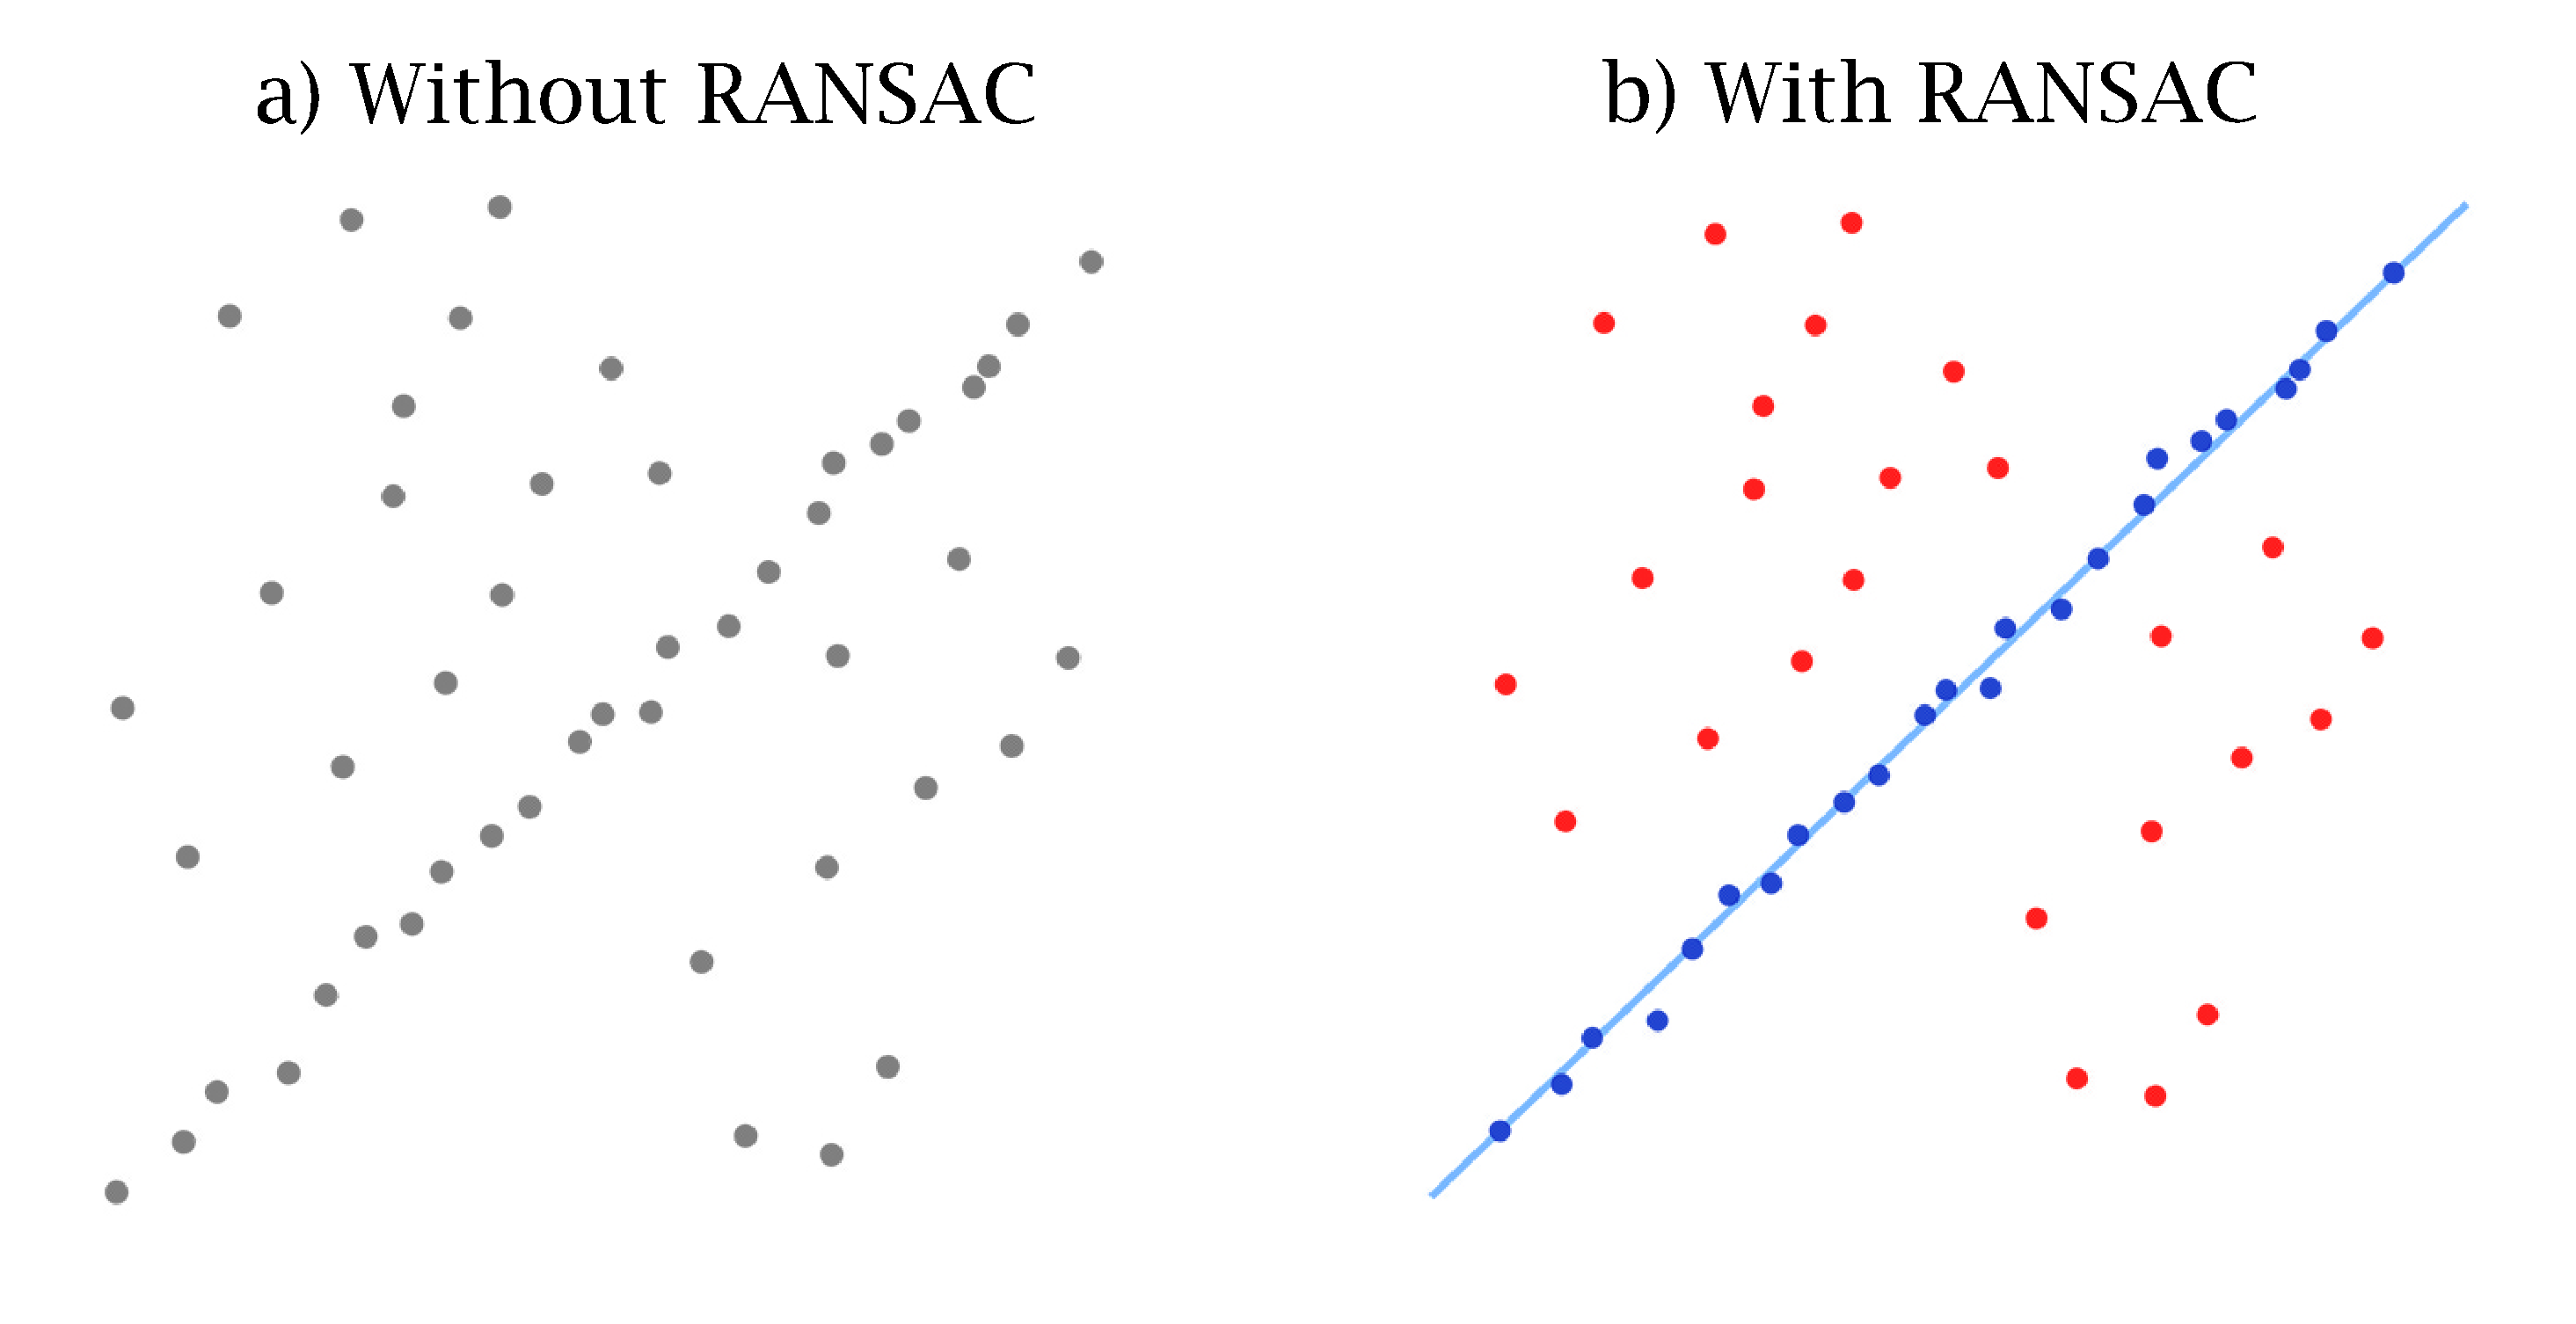
\includegraphics[width=0.8\linewidth]{figures/PDF/RANSAC.pdf}\\
        %\caption{Surroundness among connected components (b) and among borders (c)\cite{Suzuki}}
        \caption{ a) A data set without outliers and inliers distinguished\protect\footnotemark. b) The RANSAC algorithm applied to fit a line. Outliers in red are dismissed in the result\protect\footnotemark.}
        \label{fig:ransac chart}
    \end{minipage}
\end{figure}
\footnotetext[1]{\url{https://commons.wikimedia.org/wiki/File:Line_with_outliers.svg}}
\footnotetext{\url{https://commons.wikimedia.org/wiki/File:Fitted_line.svg}.}


\noindent By using RANSAC, a random subset, entirely consisting of inliers, would define the fitted line. Since the algorithm is based on the probability that a particular group of inliers should represent the fitted line, the accuracy of RANSAC is typically improved by more iterations. Except when overfitting the model, which can cause the algorithm to find a local minimum, giving poor results.


\subsubsection{Hough Transform}
The Hough Transform\cite{Duda} is a technique used to isolate simple shapes within an image. Initially, Hough Transform was created with the intent to find lines but has later been extended to identify positions of arbitrary shapes, most commonly circles and ellipses. By using a voting procedure, the purpose of Hough Transform is to identify imperfect instances of objects inside a certain class. Moreover, a simple shape is defined as one that can be represented by only a few parameters. For example, a line can be defined with two parameters: slope and intercept. A circle can be defined with three parameters: the coordinates of the center (x,y) and the radius (r).  \\

\noindent The standard Hough Transform is used for detecting lines and achieves this by describing a line in the Hesse normal form: \begin{equation} p = xcos(\theta) + ysin(\theta) \end{equation}  where $p$ is the perpendicular distance, in pixels, from the origin to the line, and $\theta$ represents the angle measured in radians, which is the orientation of $p$ as shown in \textit{Figure \ref{fig:hough graph} a)}. \\

\noindent Each line can now be represented in the ($p$, $\theta$) form, which implies that any value ($p$, $\theta$) corresponds to a line in two-dimensional parameter space. Therefore, every ($x$, $y$) value in an image can now be represented as a curve, according to \textit{Equation 2.2}. Furthermore, one can imagine this ($p$, $\theta$)-plane as the hough-space where every ($x$, $y$) value in an image are accumulated into this space. The result consists of several sinusoidal curves that cross where lines occur, as shown in \textit{Figure \ref{fig:hough graph}  b)}. Moreover, a voting procedure is used to tell where lines are in an image. For every point on a line, the corresponding accumulator cell is increased. Thereafter, finding the cells with the most peaks in the accumulator array tells where the lines are in the corresponding image. To better find the peaks in the accumulator array Hough Transform can use Morphological operations, like applying a threshold. However, different operations might yield different results depending on the image. Explanations of different morphological operations can be found in \textit{Section 2.3.2}

\begin{figure}[H]
    \centering
     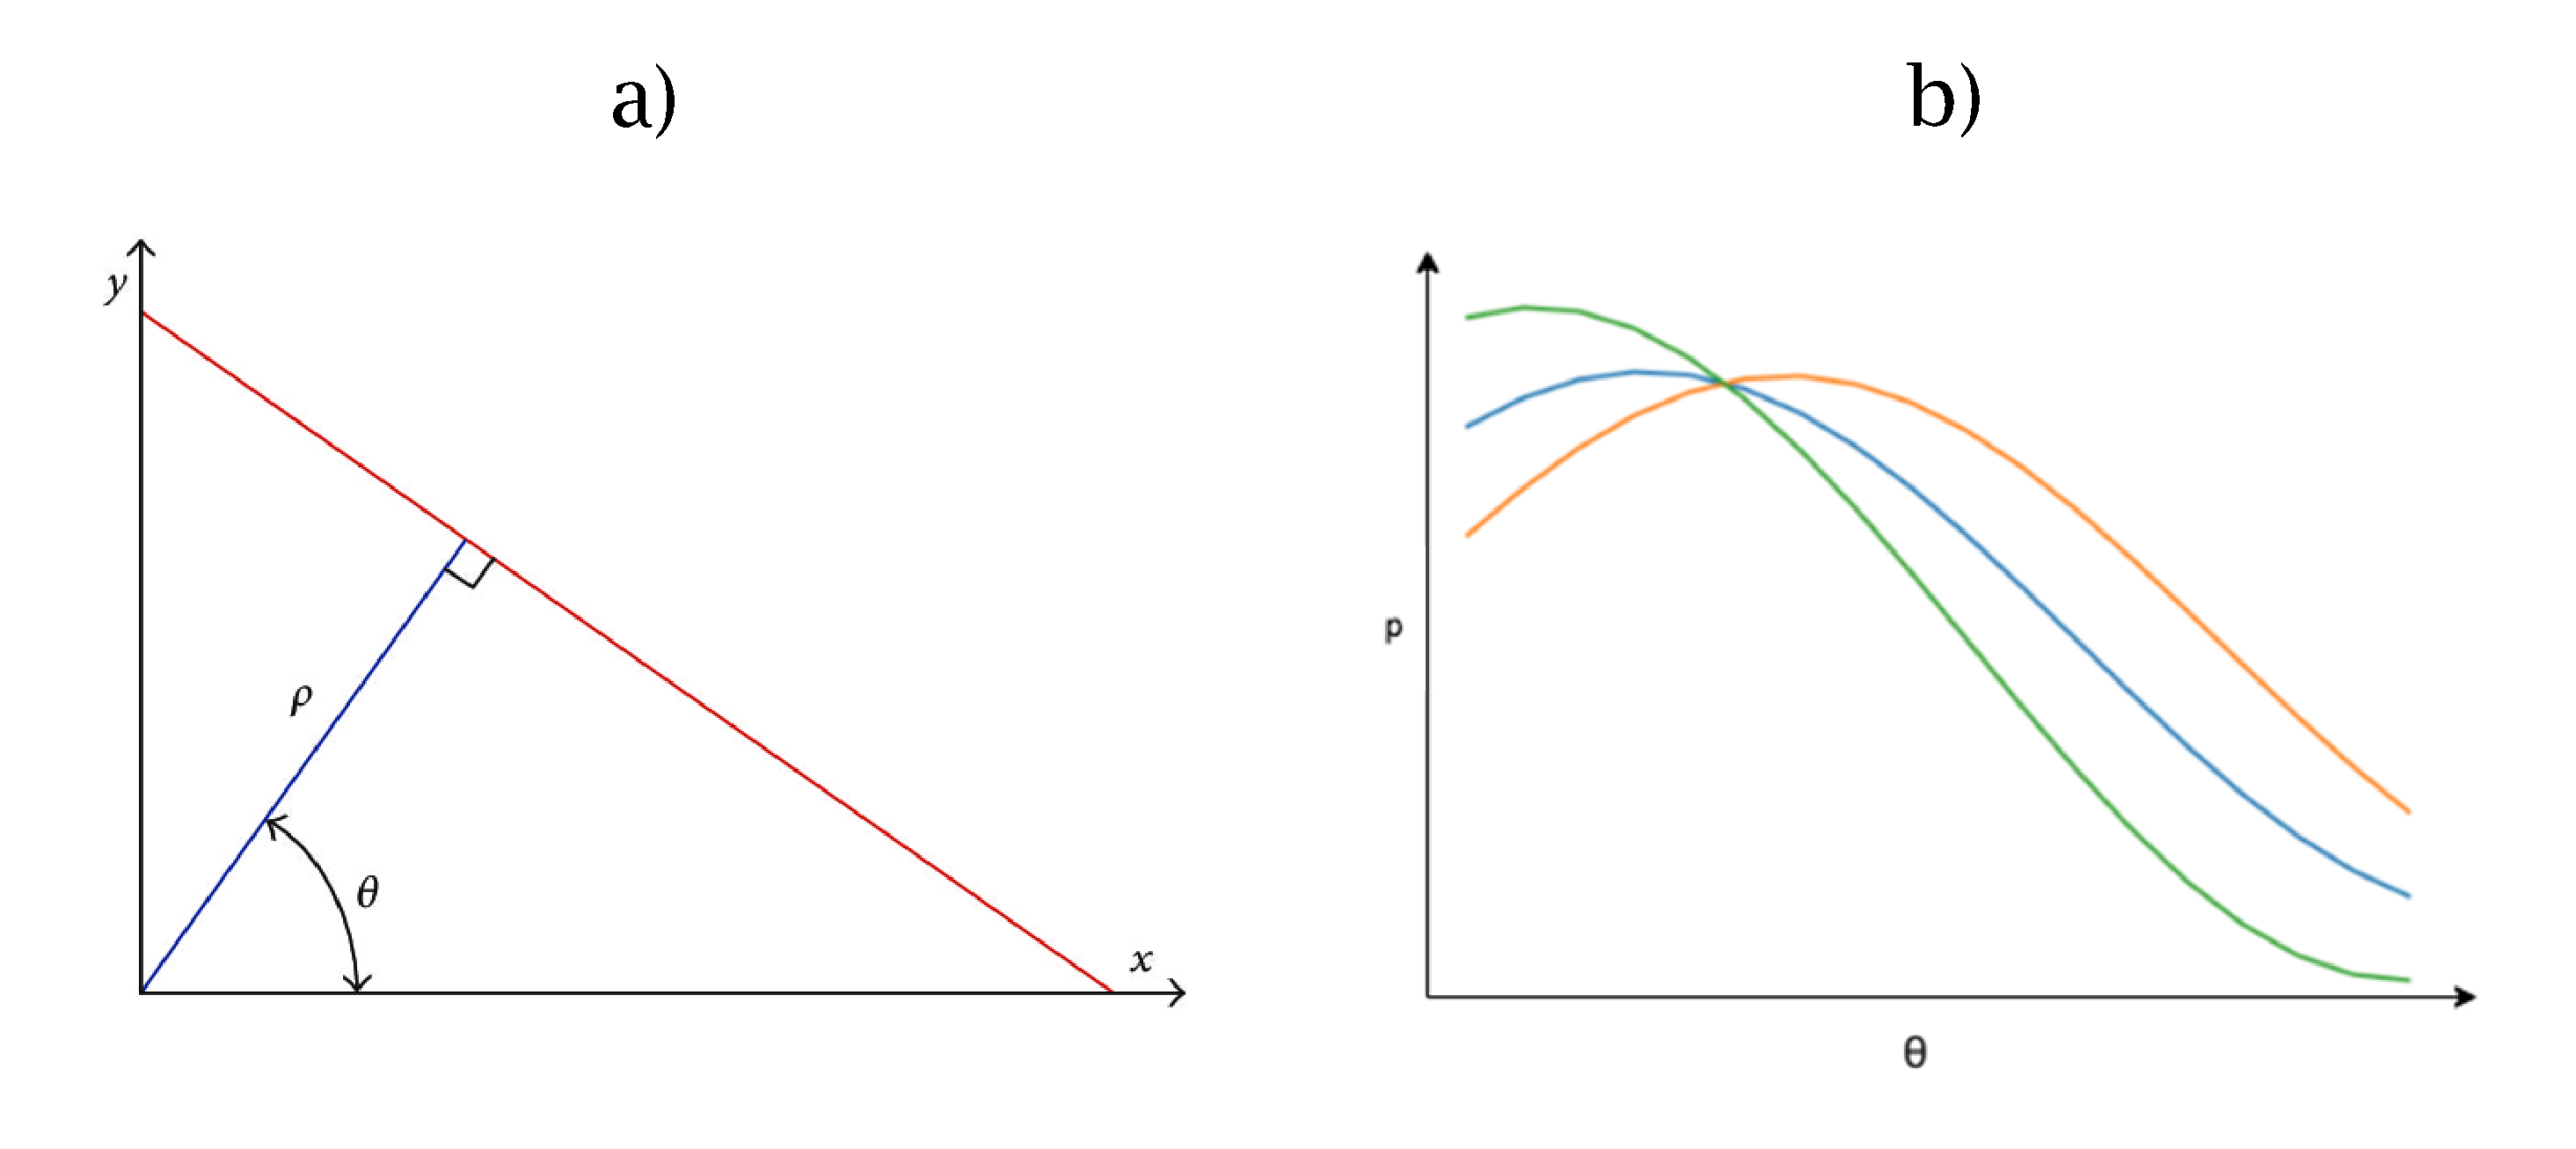
\includegraphics[width=1\linewidth]{figures/PDF/Hough_graph.pdf}\\
    \caption{a) Rho and theta parameters of a straight line\cite{Duda}. b) Three different colored curves obtained by \textit{Equation 2.2}. The intersecting point indicates a line with the parameters $p$ and $\theta$.}
    \label{fig:hough graph}
\end{figure}

\subsubsection{Modified Hough Transform}
Using modified versions of Hough Transform enables the technique to find shapes like circles and ellipses. To find circles in imperfect images, one can use Circle Hough Transform (CHT). The technique is similar to the standard Hough Transform, with the difference being that the parameter space is different. Therefore, the same procedure can be used in CHT to detect other features with other analytical descriptions. In general,  a circle can be described by: \begin{equation} {(x-a)}^2 + {(y-b)}^2 = r \end{equation} where ($r$) is the radius and ($a$, $b$) is the center of a circle. Forthwith, for every fixed ($x$, $y$) value in an image, every parameter in \textit{Equation 2.3} can be found. Therefore, the hough-space is now the ($a$, $b$, $r$)-plane. However, because the ($a$, $b$, $r$)-plane defines a three-dimensional space, the parameters can be identified in two stages. The first stage is to fix the radius to find the optimal center point in the two-dimensional parameter space. After that, the optimal radius can be derived in one-dimensional parameter space. Moreover, the computational complexity of the algorithm increases, the more parameters that exist in the parameter space. \\

%With image pre-processed with Canny, Hough Transform is used to isolate simple shapes within the image. The algorithm is divided into different parts, depending on what shape is of interest. To find the exact position of, e.g., a circular object, Circle Hough Transform looks for circular shapes using an accumulator matrix, which divides the images into groups of pixels (usually size 3x3). Following edges found using Canny, non-circular edges are ignored. Valid circular shapes are specified using parameters deciding radius interval, as well as the desired number of circles. The intersection point of the circle is later calculated, finding the center of the circle. Lastly defined and valid shapes in the image are identified and painted as seen in Figure 2. \\

%\noindent\begin{minipage}{.6\textwidth}
%  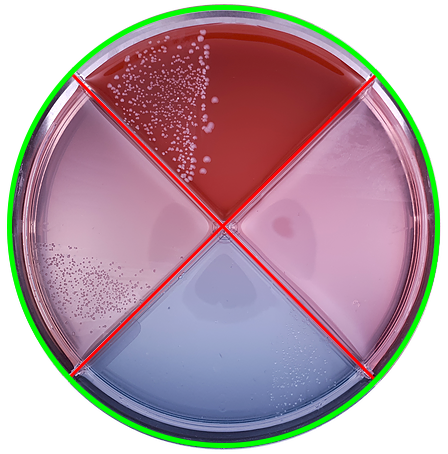
\includegraphics[width=.5\linewidth]{figures/hough.png}\\\\
%  \captionof{Fig. 2. }{Hough transformation is used to identify distinct shapes in images such as circles and lines.}
%  \label{fig:fig1}
%\end{minipage}



\subsection{Masking}
\noindent Region-of-interest (ROI) processing is an approach aiming to extract that information from a specific subregion of an image. The ROI is usually defined by points, lines, circles, or other shapes, which is then used to apply a binary mask to the image. The binary mask is created with the same size as the input image. Pixels within the ROI is set to 1 and the remaining pixels to 0. \textit{Figure \ref{fig:masking}} illustrates before and after masking, where the ROI is the agar plate. \\ 

\begin{figure}[H]
    \centering
    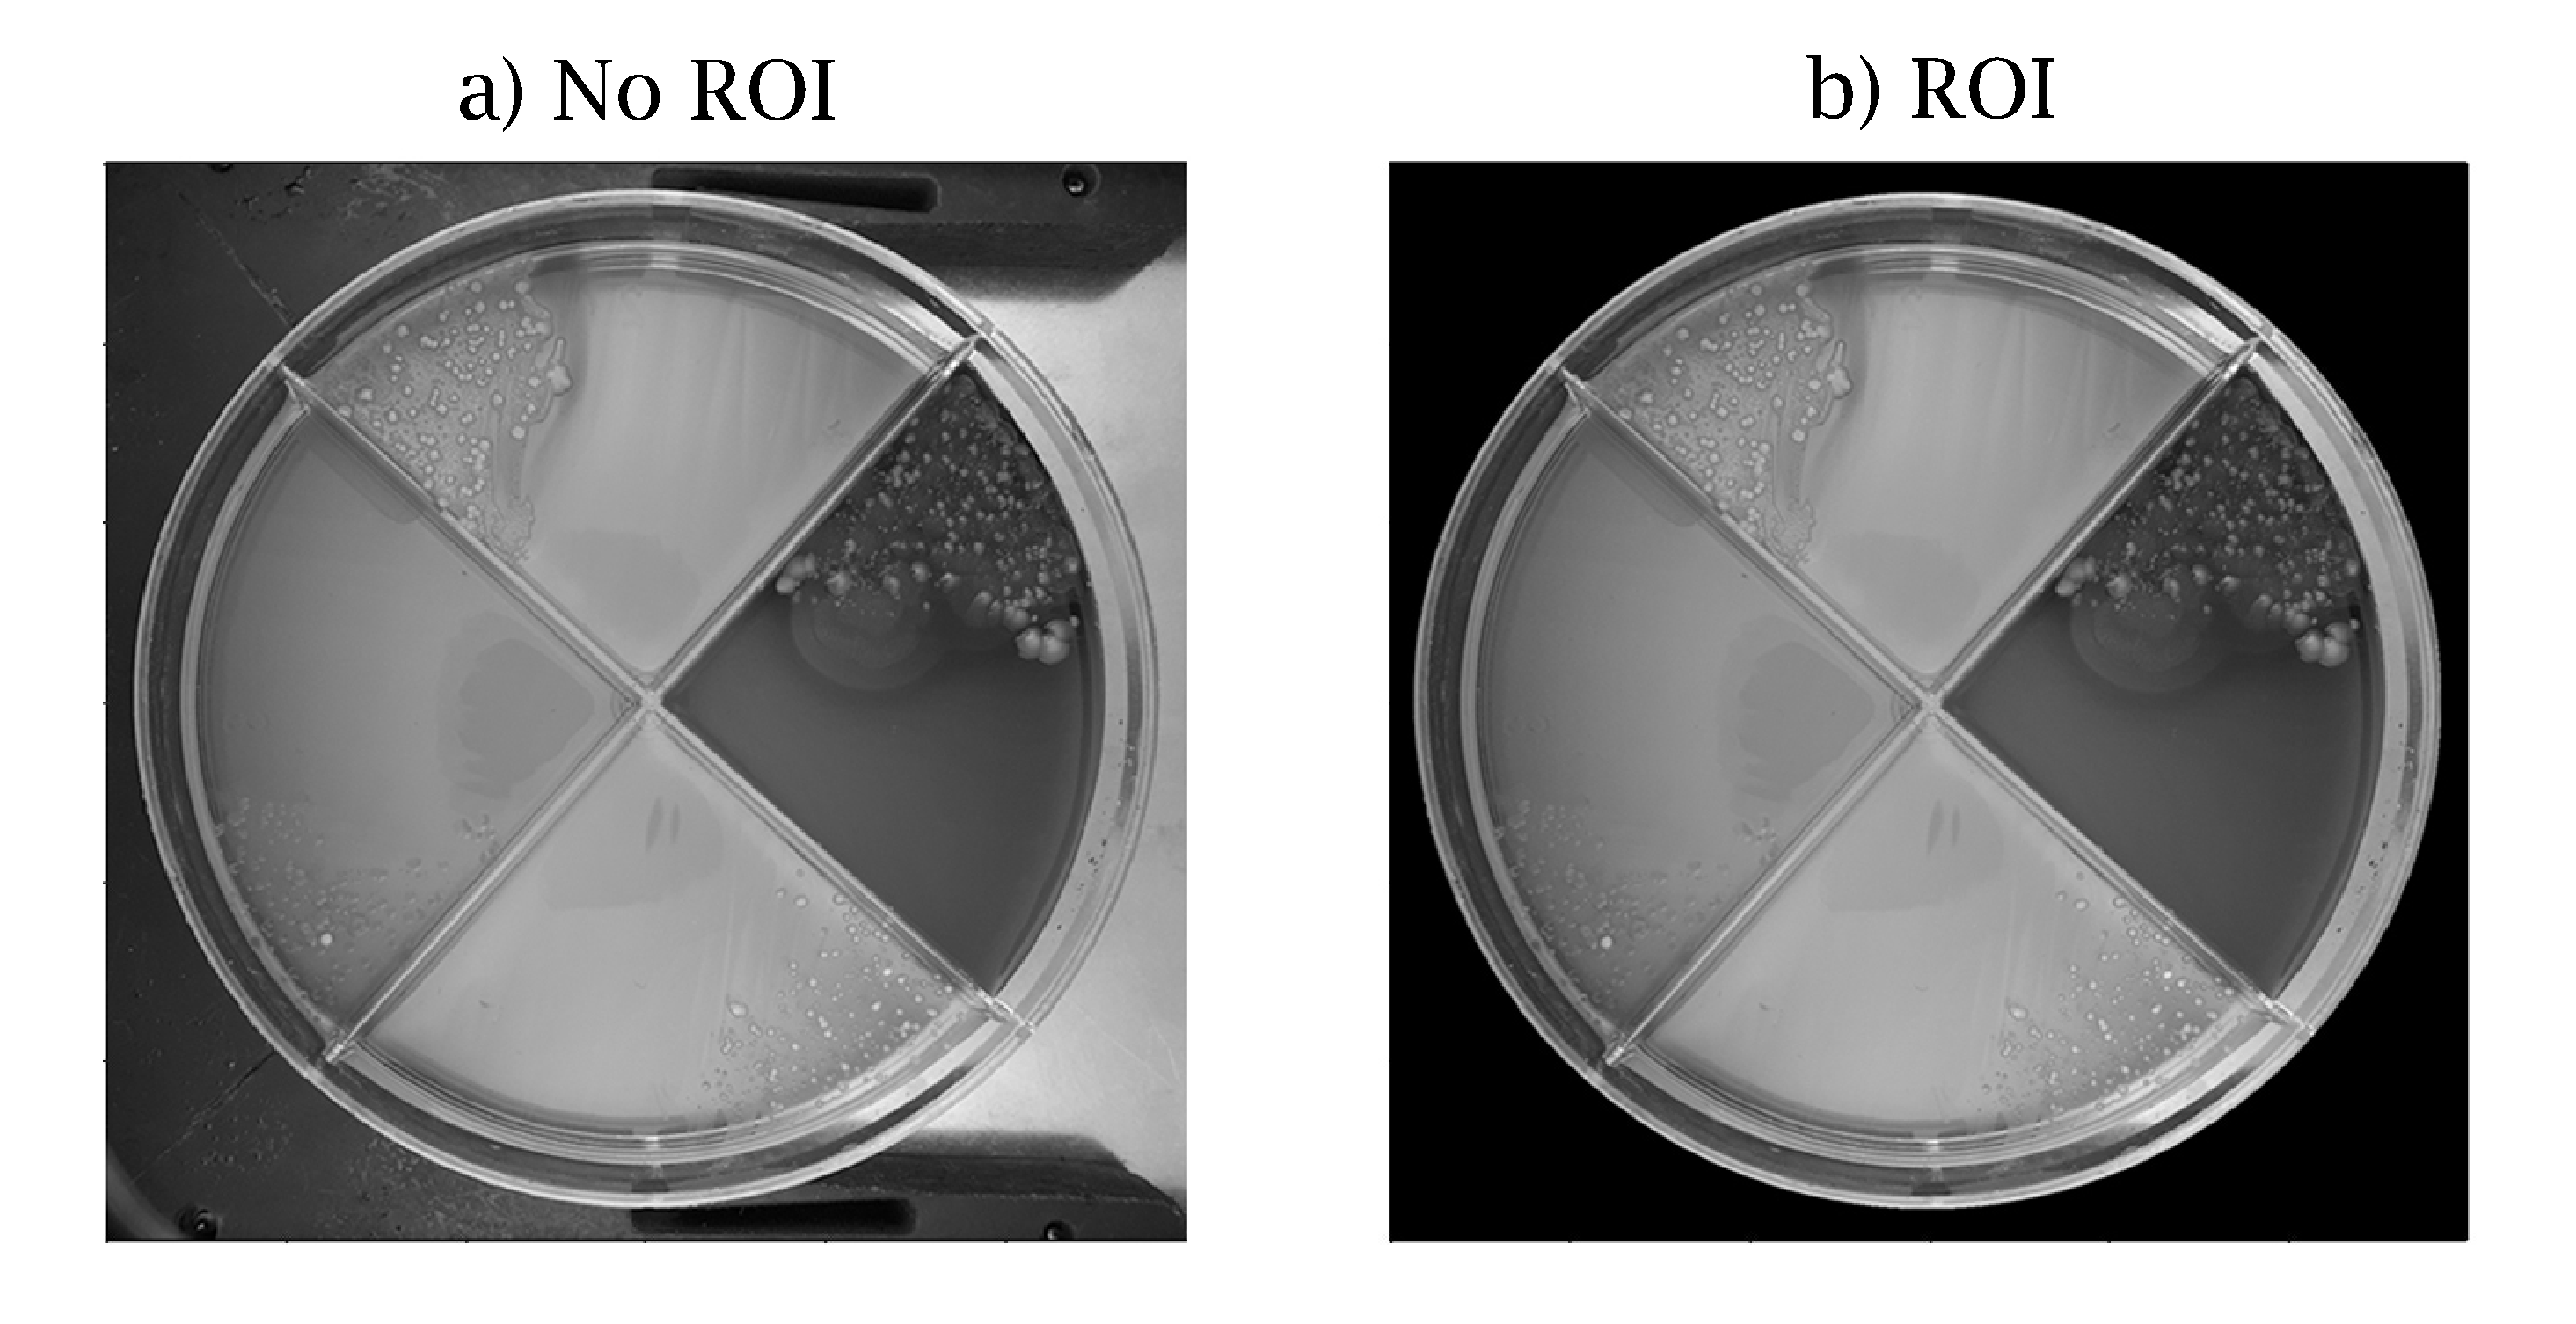
\includegraphics[width=0.8\linewidth]{figures/PDF/ROI.pdf}\\
    \caption{Figure illustrates an image with and without masking of irrelevant data using points given by \texit{Circle Hough Transform}}
    \label{fig:masking}
\end{figure}

\subsection{Color Space Image segmentation}
In circular shaped objects, it can sometimes be challenging to determine the rotation. With the human eye, one can recognize a specific shape, color, or feature within an object that only occurs in a particular direction, thus determine the rotation. This rotational landmark can be extracted using \textit{Image Segmentation}\cite{Rahmat}, which simply divides groups of pixels together based on given criteria.\\  


\noindent In \textit{Figure \ref{fig:segmentation} a)}, a compartment in distinctive red can be distinguished in the right half of the image. In order to extract the orientation data of this compartment, its pixels need to be segmented. To segment areas based on color, criteria can be defined by Color Spaces, which are colors represented of their different components, e.g., RGB (Red, Green, Blue) or HSV (Hue, Saturation, Value). For example, in \texit{Figure \ref{fig:segmentation} b), the red tones in the HSV-space are, in this case, generally more localized and visually separable. The RGB-space in \texit{Figure \ref{fig:segmentation} c)}, on the other hand, shows that the red tones have a larger span across both the green and blue axis.}
By adjusting color space values, different information can be extracted from the image. For example, changing the Red in RGB to 0 would remove all red tones in a picture, leaving only a spectrum of green and blue.\\

\begin{figure}[H]
    \centering
     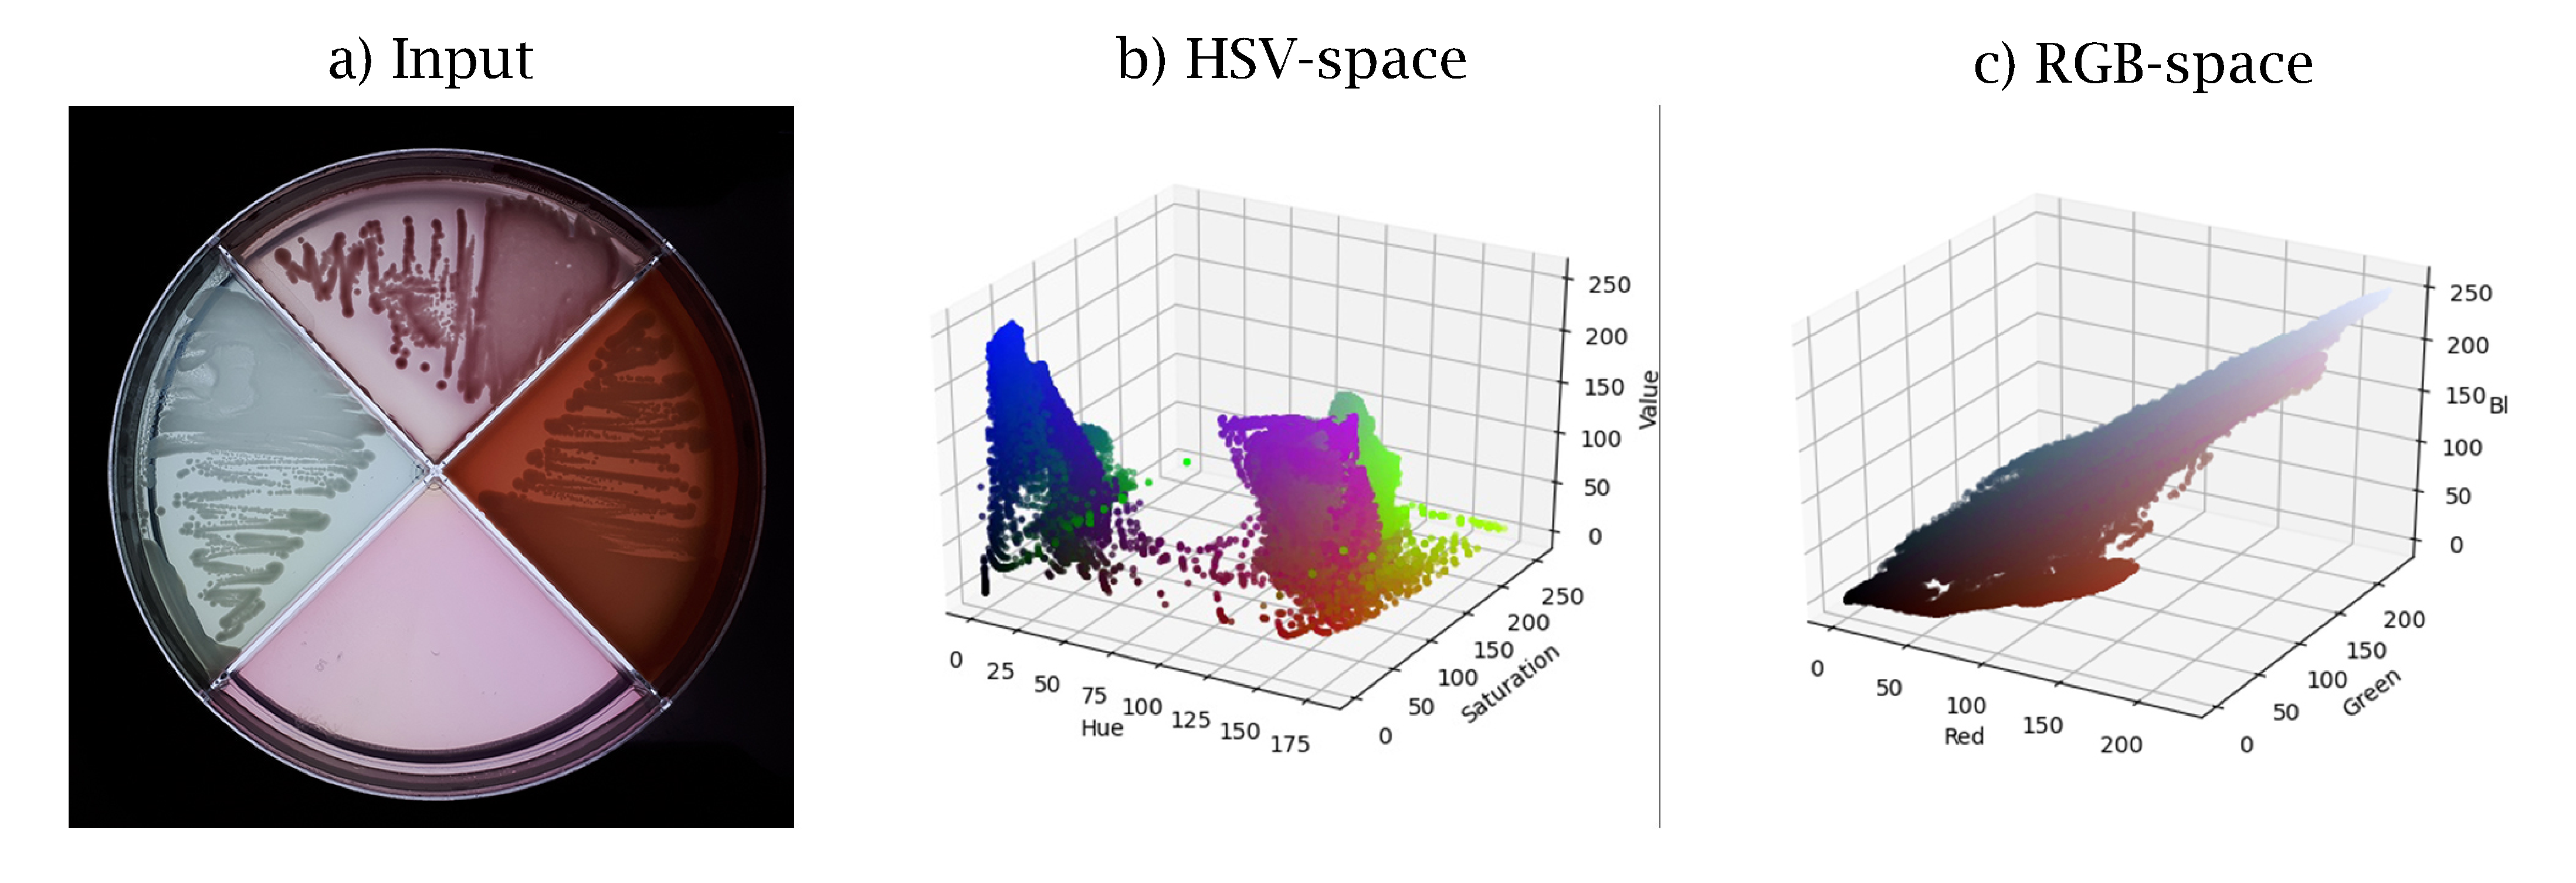
\includegraphics[width=1.1\linewidth]{figures/PDF/Color_space.pdf}\\
    \caption{{a) Example of an input image with a distinctive red-colored compartment. b) An HSV-space 3D scatter plot of the input. c) An RGB-space 3D scatter plot of the input.}}
    \label{fig:segmentation}
\end{figure}


\subsection{Image registration}
Misalignment in images is a common issue and can happen for a variety of reasons. However, the most common is due to images being captured under variable conditions, such as changes in camera perspective or the scene content. Image registration\cite{Nag} is a technique used in medical sciences, remote sensing, and computer vision that corrects misaligned images. The fundamental idea is to align two or more images of the same scene with one image designated as the reference image. Thus, getting an image matching the reference image (see \textit{Figure \ref{fig:image reg}}). There exist multiple image registration techniques, but the majority of them can be broken down into the following steps described below: \\
\begin{enumerate}
    \item \textit{Feature detection:} The detection process of different features in an image. This process can be manual or automatic; however, automatic detection is preferable. Moreover, an example of features this process looks for is edges, contours, closed-boundary regions, line intersections, and corners. Different image registration techniques can be divided into intensity-based or feature-based. Briefly, intensity-based methods look for distinctive edges in an image whereas, feature-based looks for specific objects which are more prevalent in computer vision. 
    \item \textit{Feature matching:} The process of matching the different features detected in the reference image and those detected in the non-aligned pictures (sensed images). 
    \item \textit{Transform model assessment:} The parameters of the mapping functions are estimated by aligning the sensed image with the reference image. 
    \item \textit{Image transformation:} The sensed image is transformed by employing the mapping functions.
\end{enumerate} 
\ \\
\noindent The tasks described above have typical problems, and problems might occur if specific requirements are not obtained\cite{Zitova}. The detection of features should be distinctive objects or objects spread over the image, which are easily detectable. Moreover, the feature matching between the sensed image and the reference image needs to have enough common features to achieve proper registration. Especially, on occasions when the images do not cover the same scene, object collision occurs or other unexpected changes. \\

\begin{figure}[H]
    \centering
     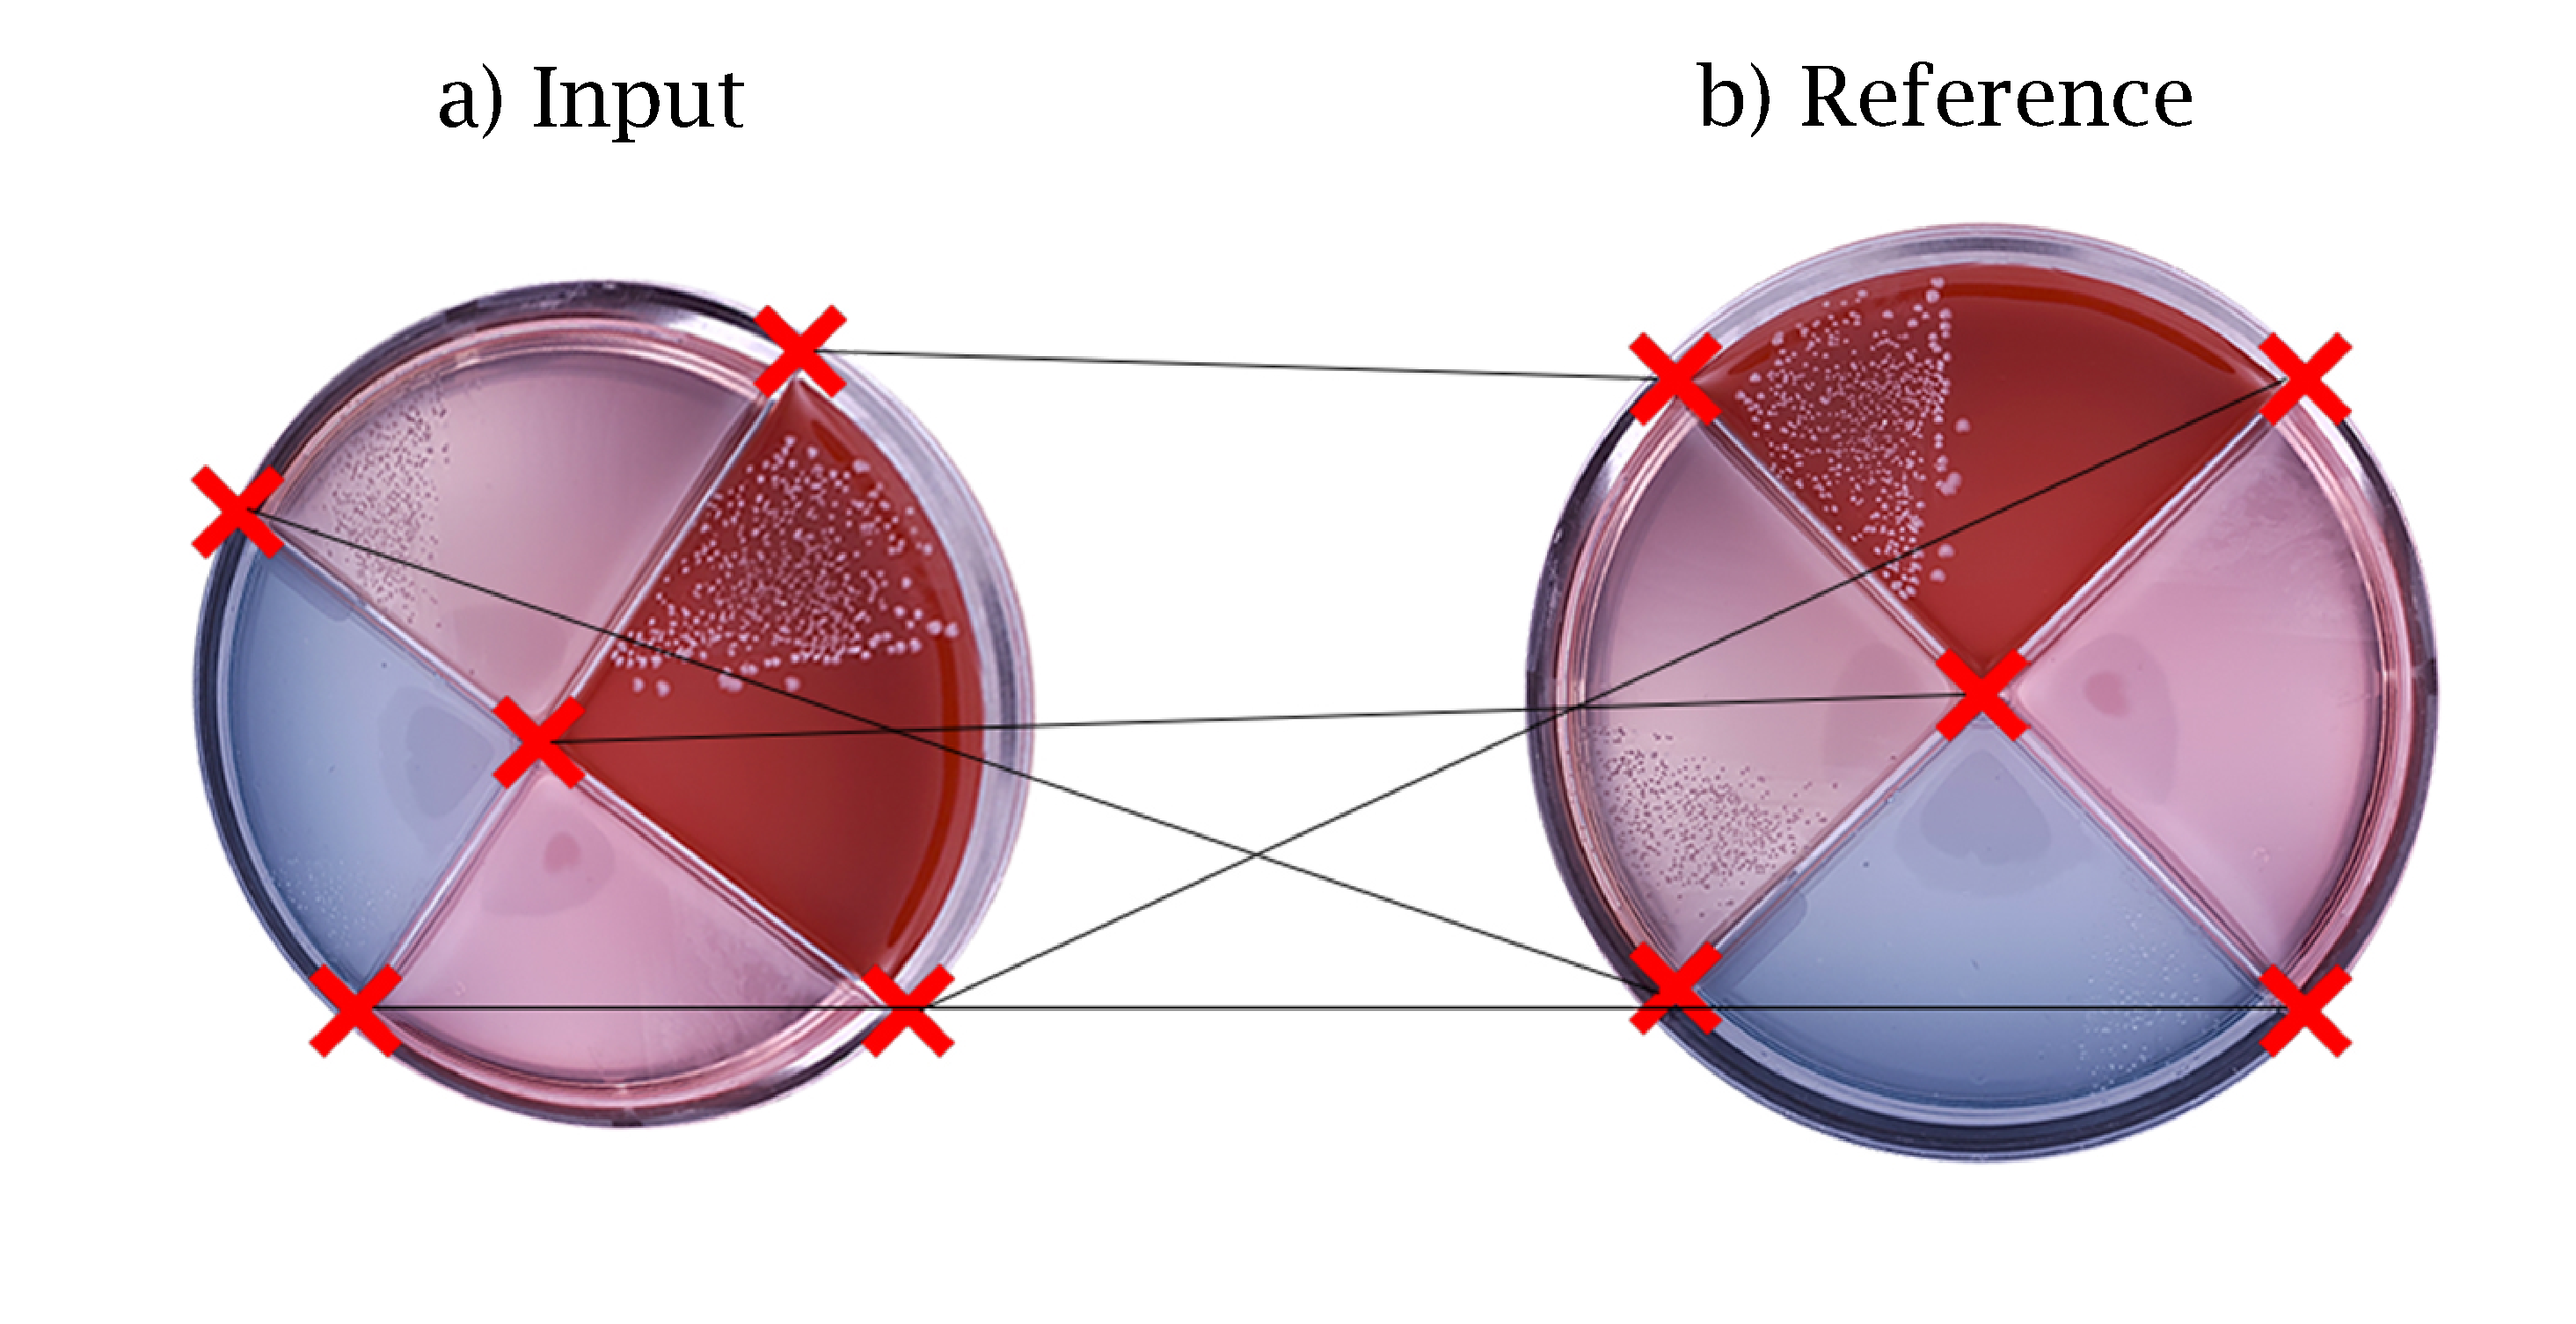
\includegraphics[width=0.8\linewidth]{figures/PDF/Image_reg_theory.pdf}\\\\
    \caption{a) Will be adjusted to mimic the reference image in b) as close as possible, based on the reference points}
    \label{fig:image reg}
\end{figure}

\subsubsection{Different transformation models}
Different image registration techniques\cite{Nag} can also be classified depending on what transformation models they use. The most used are linear transformations followed by projective transformations. However, there also exist non-linear transformations, but it is beyond the scope of this work. Linear transformations include transformation on rotation, translation, scaling, and shearing in images, and are collectively known as affine transforms. The transformation in a two-dimensional space is done by determining the transformation matrixes shown below: \\

\noindent\begin{enumerate}
    \item \textit{Rotation:}  object can be rotated given an angle $\theta$ proportionate to its origin.  \begin{equation} \begin{bmatrix} x_{1} \\ y_{1} \end{bmatrix} = \begin{bmatrix} cos\theta & sin\theta \\ -sin\theta & cos\theta \end{bmatrix} + \begin{bmatrix} x_{2} \\ y_{2} \end{bmatrix} \end{equation} $(x1, y1)$ is the new point, $(x2, y2$) is the old point, and $\theta$ is the rotation parameter. \\
    \item \textit{Scaling:} Scaling is done to resize an image or to match images with different sizes.  \begin{equation} \begin{bmatrix} x_{1} \\ y_{1} \end{bmatrix} = \begin{bmatrix} s_{x} & 0 \\ s_{y} & 0 \end{bmatrix} + \begin{bmatrix} x_{2} \\ y_{2} \end{bmatrix} \end{equation} Where $(x1, y1)$ is the new point, $(x2, y2)$ is the old point, and $(s1, s2)$ is the scaling parameters. For example, if $s1 = 2$ and $s2 = 2$ the old point $(x2, y2)$ is scaled by two in every direction. \\
    \item \textit{Translation:} If a point x,y  is to be translated by t units then, the transformation matrix is: \begin{equation} \begin{bmatrix} x_{1} \\ y_{1} \end{bmatrix} = \begin{bmatrix} x_{2} \\ y_{2} \end{bmatrix} + \begin{bmatrix} t_{1} \\ t_{2} \end{bmatrix} \end{equation} where $(x1, y2)$ is the new point, $(y2, x2)$ is the old point, and $(t1, t2)$ is the translation value. \\
    \item \textit{Shearing:} Shearing slants the shape of an object. There exist two sheering transformations, x-shear, which changes the values of the coordinates and y-shear, which changes the values of the y coordinates.  \begin{equation} \begin{bmatrix} x_{1} \\ y_{1} \end{bmatrix} = \begin{bmatrix} a_{11} & a_{12} \\ a_{21} & a_{22} \end{bmatrix} \begin{bmatrix} x_{2} \\ y_{2} \end{bmatrix} + \begin{bmatrix} a_{13} \\ a_{23} \end{bmatrix}  \end{equation} where $(x1, y2)$ is the new point, $(x2, y2)$ is the old point, and $(a_{11}, a_{12}, a_{21}, a_{22}, a{13}, a{23}$ is the sheering parameters.  \\
    \item \texit{Reflection:} Reflection is done by mirroring an image of the original object. Simply, reflection does not change the size of the object. 
\end{enumerate}
\ \\
\noindent The difference between linear transformations and projective transformations is that linear transformations are global by nature. Therefore, the geometrical difference between images cannot be modeled. However, projective transformations allow for warping a target image to match a reference image, which is achieved by a homography. A homography is a transformation matrix that maps points from the target image to the corresponding point in the reference image as follows:  \begin{equation} \begin{bmatrix} x_{1} \\ y_{1} \\ 1 \end{bmatrix} = H \begin{bmatrix} x_{2} \\ y_{2} \\ 1 \end{bmatrix} =  \begin{bmatrix} h_{00} & h_{01} & h_{02} \\ h_{10} & h_{11} & h_{12} \\ h_{20} & h_{21} & h_{22} \end{bmatrix} \begin{bmatrix} x_{2} \\ y_{2} \\ 1 \end{bmatrix} \end{equation} Where H is the homography matrix.  

\subsection{Image accuracy validation}
When working with large datasets, manual validation of each output may be too time-consuming and a waste of resources. By automating the validation process for each output, higher accuracy can be achieved as well as saving time otherwise spent on debugging.  \\

\noindent For shape oriented image processing, different types of \textit{Image moment}\cite{Huang}\cite{Chaumette} algorithms can be used. Image moments are values of the weighted average of pixel intensities in images, which can then be used to compare two images. The moment of a single-channel binary image, for example, is defined as \textit{Equation 2.9}, with I(x, y) being the intensity of a pixel on a given x,y coordinate. \begin{equation}
    M = \sum_x \sum_y{I(x, y)}
\end{equation} The formula can be extended to consider both pixel intensity, as well as its position in the image using \textit{Equation 2.10}. However, this method is not entirely transformational invariant.\\ \begin{equation}
    M_i_j = \sum_x \sum_y{x_iy_jI(x, y)}
\end{equation} 

\noindent As an extension to image moments, \textit{Central moments} can be used to address translation and scale-varieties. The central moment is defined using \textit{Equation 2.11}. Where $\overline{x}$ and $\overline{y}$ are the weighted averages of pixels constituting different shapes (or blobs) found in an image.\\

\begin{equation}
    \mu_i_j = \sum_x \sum_y{(x - \bar{x})^i(y - \bar{y})^jI(x, y)}
\end{equation}  
 
\noindent For the moments to be scale-invariant, the \textit{Normalized Central Moments} are calculated as follows in \textit{Equation 2.12.}\\
\begin{equation}
    \eta_i_j = \frac{\mu_i_j}{(i+j)/2+1}
\end{equation} 
 
\noindent Even though the normalized central moments are translation and scale-invariant, rotation is still something to take into consideration. An algorithm called Hu Moments addresses this problem using a set of 7 values. Each value is calculated using Normalized Central Moments, where the first six moments address translation, scale, rotation, and reflection, and the last moment is skew invariant, which can identify mirror images.





%%%%%%%%%%%%%%%%%%%%%%%%%%%%%%%%%%%%%%%%%%%%%%%%%%%%%%%%%%%%%%%%%%%%%%
%%% lorem.tex ends here

%%% Local Variables: 
%%% mode: latex
%%% TeX-master: "demothesis"
%%% End:
